% !Mode:: "TeX:UTF-8" 

\BiChapter{克隆代码变化时一致性维护需求预测方法}
{Predicting Clone Consistency-Requirement at Clone Changing Time}

\BiSection{引言}
{Introduction}

由于日益增长的软件开发的需求,软件中存在大量的由开发人员复用既有代码所产生的克隆代码。在随着软件系统演化的过程中,克隆组内的某一克隆代码片段可能会被软件开发员修改而发生变化。同时,由于克隆组内的克隆片段的相似性,该克隆片段的变化可能会导致其所在克隆组在未来演化过程中发生一致性变化。遗忘这种克隆代码的一致性变化,会引入与之相关的克隆一致性缺陷,从而增大系统的维护代价。本章将由克隆代码变化所导致的其所在克隆组未来演化过程中发生的一致性变化,称为克隆代码变化时的一致性维护需求。在克隆代码变化时时预测克隆代码的一致性维护需求,可以帮助避免克隆代码的一致性缺陷,从而帮助提高软件质量和可维护性。

鉴于此,本章与第三章相似,在定义克隆代码变化时的一致性变化和一致性维护需求的基础上,使用机器学习方法在克隆代码变化时预测其一致性维护需求。为训练克隆代码变化时一致性预测模型,首先通过构建软件系统的克隆家系来收集系统中所有的克隆变化实例(发生变化的克隆代码)。然后,提取了代码属性、上下文属性和演化属性三组属性值表示克隆代码变化实例。最后,训练机器学习模型预测克隆代码变化时的一致性维护需求。在四个开源软件系统上对本章方法进行了评估,实验结果表明本章方法以合理的精确率和召回率有效地预测克隆代码变化时的一致性维护需求。本章所提出的预测方法同样可以帮助开发人员在克隆代码变化时预测克隆代码的一致性,避免克隆变化导致的一致性缺陷,从而提高软件质量和可维护性。

\BiSection{克隆代码变化时一致性维护需求}
{Clone Changing Consistency-Requirement}

\BiSubsection{克隆一致性变化实例}
{An Example of Clone Consistent Change }

在软件开发过程中,通过复用既有代码会向软件系统中引入大量的克隆代码。有研究表明软件中的克隆代码可以占到系统代码规模的7\%-23\%\cite{koschke2007survey}。与此同时,软件中存在的克隆代码不是静止不变的,会随着软件系统进行演化,其演化过程可使用克隆家系进行描述\cite{kim2005empirical}(克隆演化见本文~\ref{ref-evolution}~节)。克隆组内的某一克隆代码片段可能会被程序开发人员修改,从而引发克隆代码的一致性变化\cite{saha2011automatic}。
本文第二章通过分析克隆演化特征发现,克隆代码的一致性变化往往多于不一致性变化,因此开发人员需要警惕发生变化的克隆代码,并且当发生变化时需要考虑克隆代码的一致性问题。(具体可参考本文~\ref{ref-characteristics}~节)。

演化中的克隆变化使得克隆代码变得越来越难以维护,而克隆代码的一致性问题会导致额外的维护代价。当克隆代码发生变化时,程序开发人员需要验证克隆代码的一致性,从而导致维护代价的增加;如果开发人员忘记验证克隆代码的一致性,则可能会向系统中引入新的克隆一致性缺陷在\cite{bettenburg2009empirical} \cite {juergens2009code}。本文第三章研究了克隆代码创建时的一致性维护需求问题,在克隆代码产生时预测克隆代码一致性。在一定程度上可以降低软件的维护代价。但是,值得注意的是,并不是所有的克隆代码都可以被避免。更为重要的是,上述方法也无法处理系统中已经存在的克隆代码的一致性变化问题。因此,对系统中已经存在的克隆代码,本章将讨论克隆代码变化时其一致性维护需求问题。

在详细论述本章方法之前,先给出一个克隆代码的一致性变化的具体例子,如图~\ref{changingexamplea}~和~\ref{changingexampleb}~所示。该一致性变化例子来自于软件系统jEdit中。在图~\ref{changingexamplea}~中给出了$ 3.1.0 $版本中的两个克隆代码片段,它们之间是彼此相似的,可称之为克隆代码。在随着系统演化至$ 3.2.0 $版本时,上述两个克隆代码发生了一致性变化。具体地,$ 3.1.0 $版本中的第9-12行和第15行代码在下一版本$ 3.2.0 $中被开发人员修改。第9-12行,开发人员将{\tt selectionEnd}更改为$ 0 $,并删除了一对花括号。在第15行,开发人员删除了声明语句。如图~\ref{changingexampleb}~所示,这两个被修改的代码片段仍然是彼此相似的克隆代码(仍存在于版本$ 3.2.0 $中的同一克隆组中)。假设程序人员没有对上述两个克隆代码进行一致性维护,这必然会导致克隆代码的一致性缺陷,从而降低软件质量。

\begin{figure}[htbp]
\centering
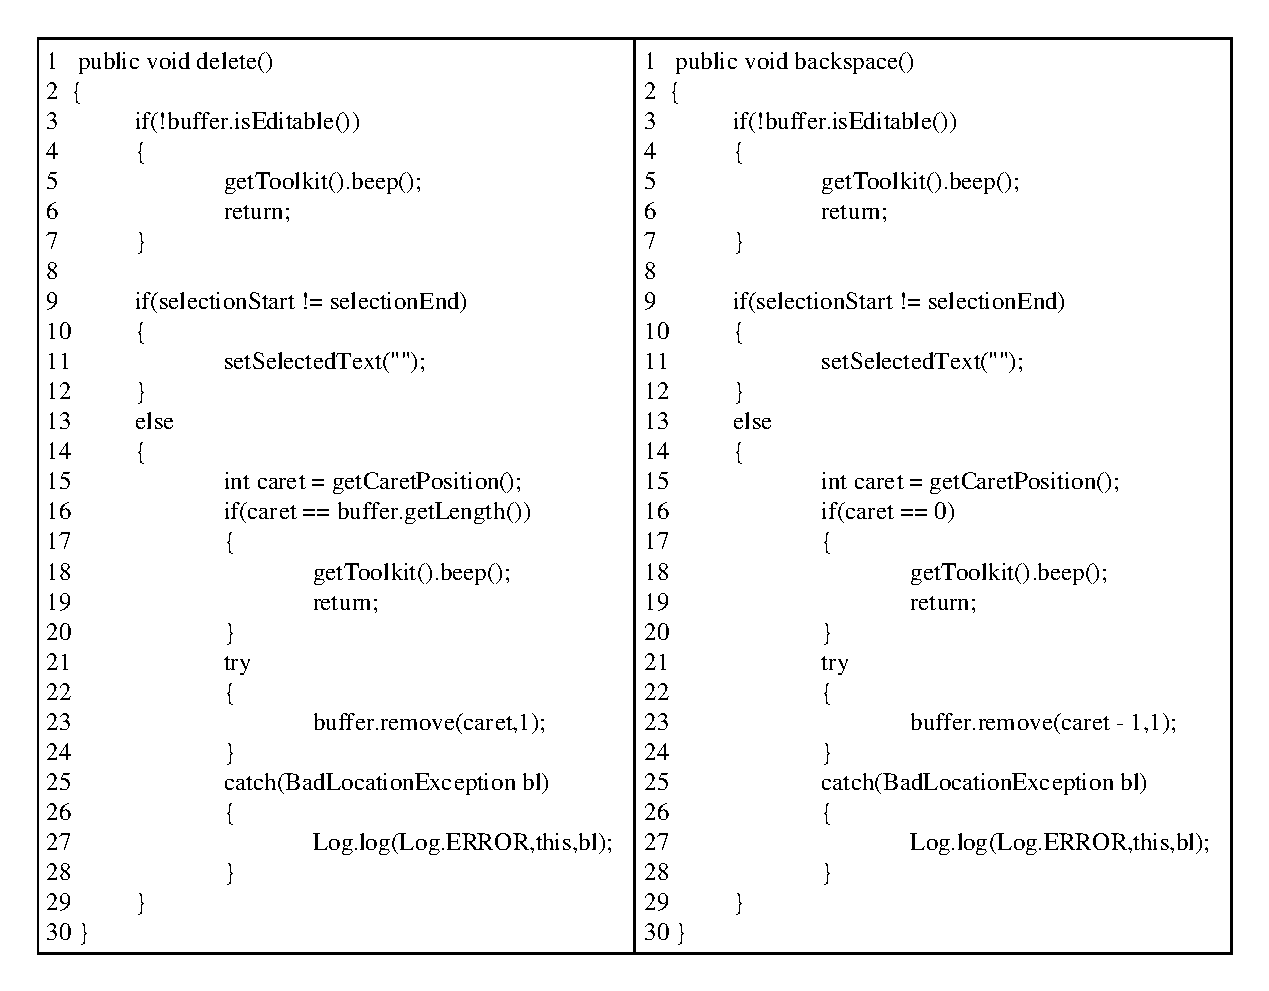
\includegraphics[width=0.8\textwidth]{co-changea.pdf}
\bicaption[changingexamplea]{}{版本$ 3.1.0 $中同一一个克隆组中的两个克隆片段}
{Fig.$\!$}{Two clone fragments in one clone group in version $3.1.0$}
\vspace{-1em}
\end{figure}

\begin{figure}[htbp]
\centering
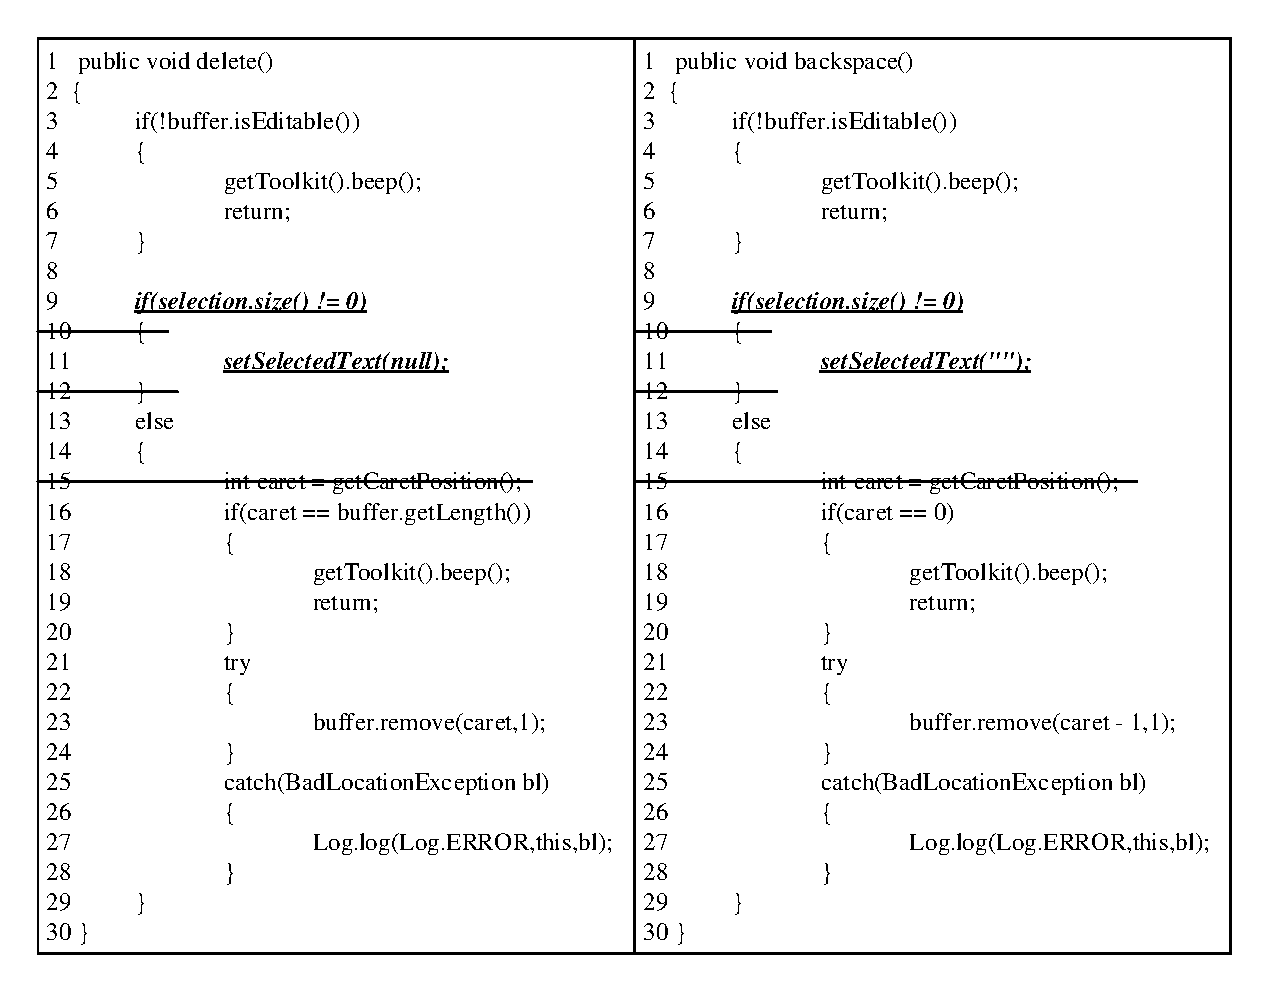
\includegraphics[width=0.8\textwidth]{co-changeb.pdf}
\bicaption[changingexampleb]{}{版本$ 3.2.0 $中克隆组中的两个克隆片段}
{Fig.$\!$}{Two clone fragments in clone group in version $3.2.0$}
\vspace{-1em}
\end{figure}

%%%图的合并
%%%%在详细论述本章方法之前,本文先给出一个克隆代码的一致性变化的具体例子,如图~\ref{co-change}~所示。该一致性变化例子来自于软件系统jEdit中。在图~\ref{cg1}中给出了$ 3.1.0 $版本中的两个克隆代码片段,它们之间是彼此相似的,可称之为克隆代码。在随着系统演化至$ 3.2.0 $版本时,上述两个克隆代码发生了一致性变化。具体地,$ 3.1.0 $版本中的第9-12行和第15行代码在下一版本$ 3.2.0 $中被开发人员修改。第9-12行,开发人员将{\tt selectionEnd}更改为$ 0 $,并删除了一对花括号。在第15行,开发人员删除了声明语句。如图~\ref{cg2}~所示,这两个被修改的代码片段仍然是彼此相似的克隆代码(仍存在于版本$ 3.2.0 $中的同一克隆组中)。假设程序人员没有对上述两个克隆代码进行一致性维护,这必然会导致克隆代码的一致性缺陷,从而降低软件质量。
%%%%
%%%%\begin{figure}[htbp]
%%%%\centering
%%%%\subfigure{\label{cg1}}
%%%%\addtocounter{subfigure}{-2}
%%%%\subfigure[Two clone fragments in one clone group in version $3.1.0$]
%%%%{\subfigure[版本$ 3.1.0 $中同一一个克隆组中的两个克隆片段]{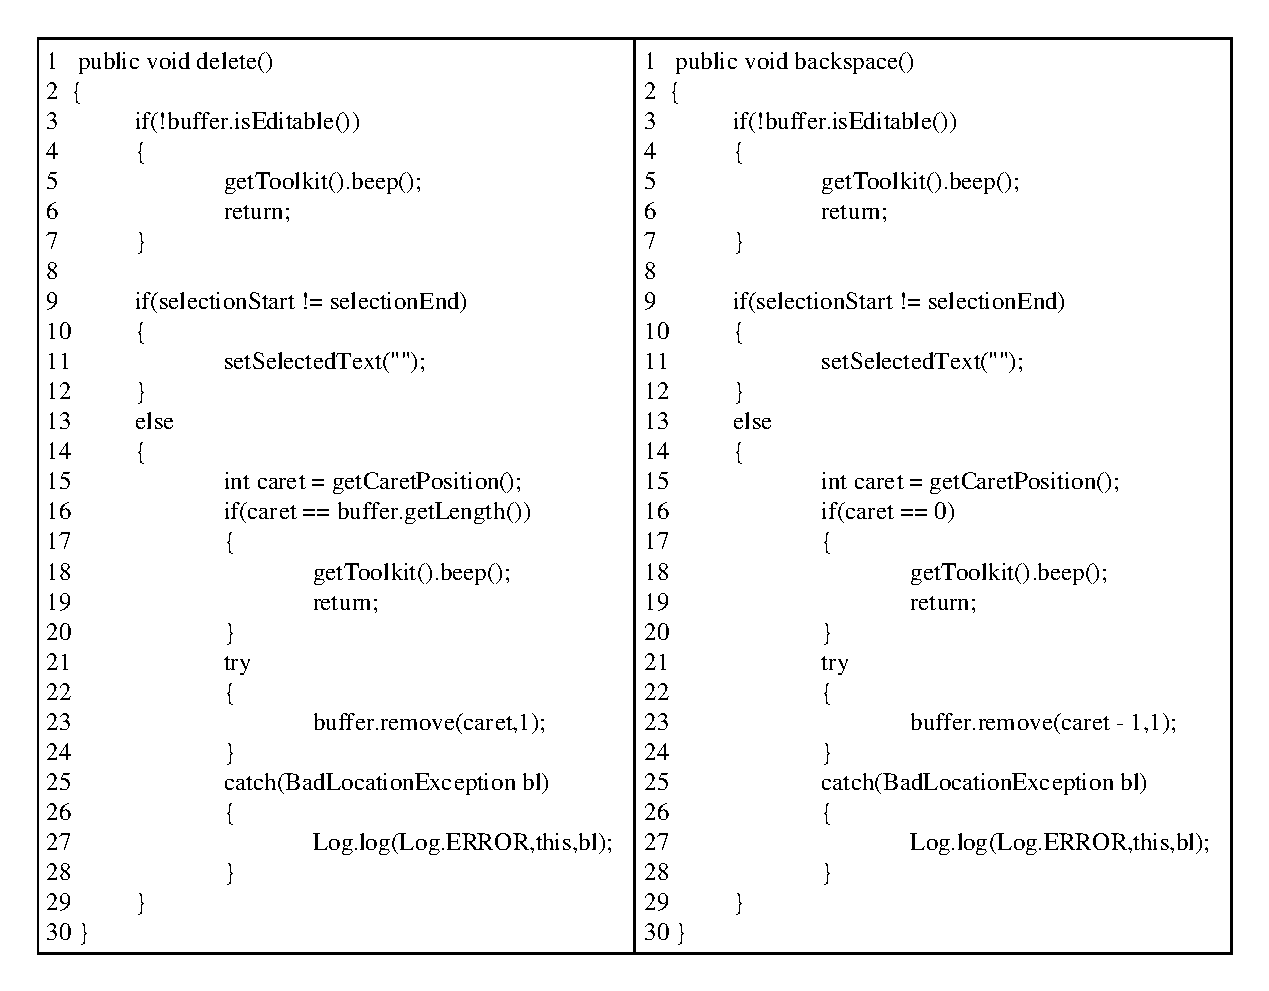
\includegraphics[width=0.8\textwidth]{co-changea.pdf}}}
%%%%\subfigure{\label{cg2}}\addtocounter{subfigure}{-2}
%%%%\subfigure[Two clone fragments in clone group in version $3.2.0$]
%%%%{\subfigure[版本$ 3.2.0 $中克隆组中的两个克隆片段]{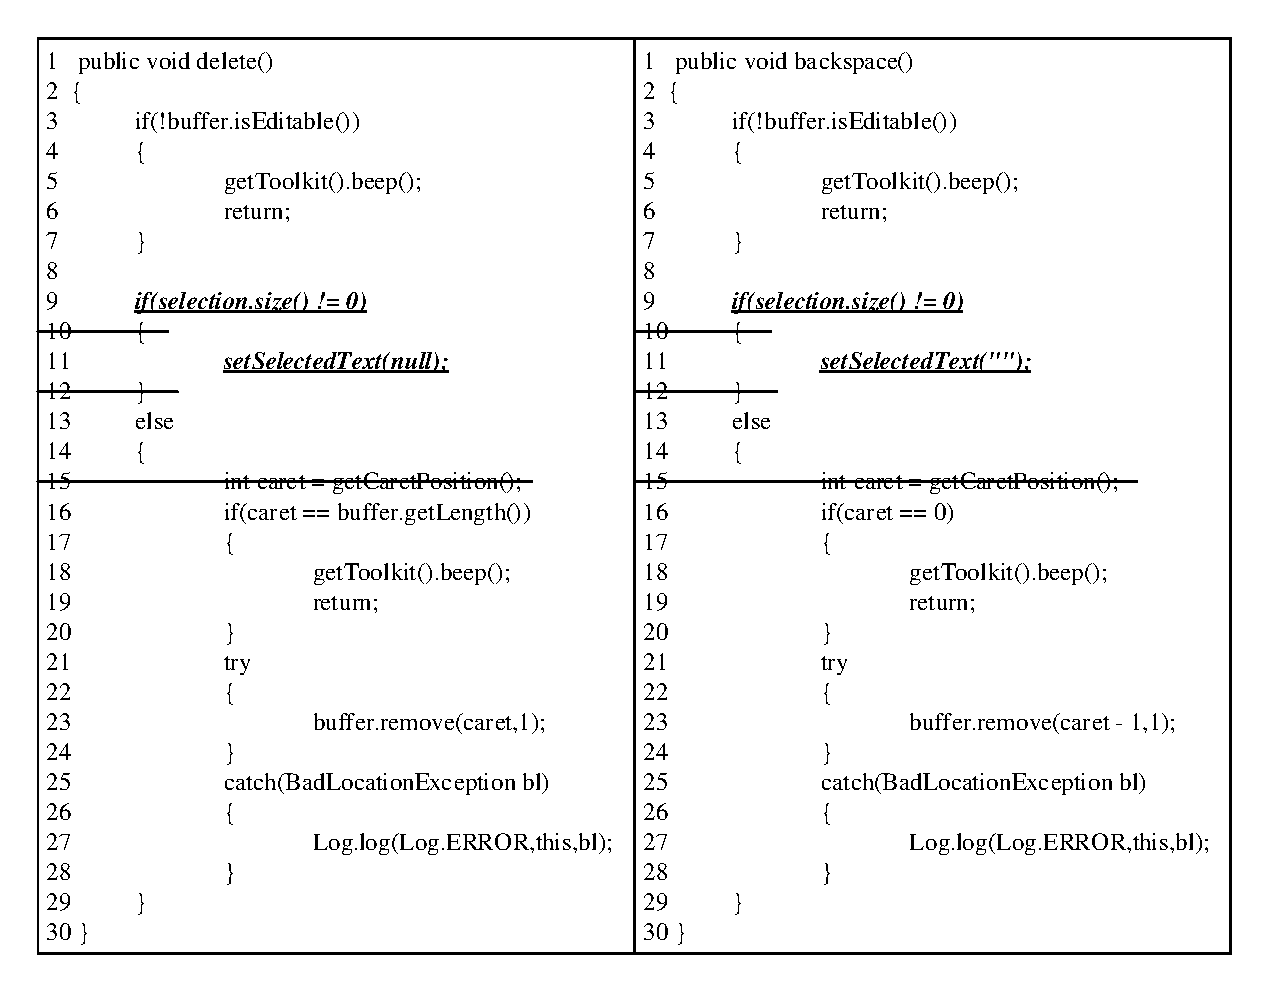
\includegraphics[width=0.8\textwidth]{co-changeb.pdf}}}
%%%%\bicaption[co-change]{}{jEdit中的一致性变化的例子}
%%%%{Fig.$\!$}{An example of consistent change from jEdit}
%%%%\vspace{-1em}
%%%%\end{figure}

鉴于此,本章对发生变化的克隆代码进行预测,在克隆代码变化时,预测克隆代码的一致性维护需求。本章在克隆代码演化的基础上结合克隆代码一致性维护,首先给出了一种克隆代码变化时的一致性变化和一致性维护需求的定义,可以帮助预测克隆变化的一致性维护需求。然后,在第二章研究的基础上重新设计了代码属性、上下文属性和演化属性三组属性表示克隆代码的变化实例。最后,使用五种不同的机器学习方法在克隆代码变化时预测其一致性维护需求。本章方法可以帮助程序开发人员避免克隆一致性缺陷,从而降低克隆代码的一致性维护代价。

%在我们的工作中,我们使用克隆检测工具{\em NiCad}来检测来自软件库的克隆。本文使用NiCad检测克隆代码(包含Type 1、Type 2和Type 3克隆代码),并使用 {\em Unique Percentage Items (UPI)}来计算克隆片段之间的相似度\cite{roy2008nicad}。这里,如果两个(或更多个)克隆片段足够相似,则它们形成克隆组。在{\em NiCad}中,这种相似性度量用UPI(代表{\em unique percentage items})表示。UPI根据代码的百分比定义了两个克隆片段之间的{\em 差异}。例如,值为$ 0.3$的UPI表示这两个克隆片段中的30\%不同;换句话说,它们中的70\%具有相同的代码行。
%在这项工作中,{\em  我们设置一个阈值$tau-{CG}$为$0.3$形成克隆组};即,如果UPI $(c_1, c_2)- 0.3$,两个克隆片段$ c_1 $和$ c_2 $被视为属于同一克隆组。}

\BiSubsection{克隆变化时一致性维护需求定义}
{The Definitions for Clone Changing Consistency-Requirement}

在克隆代码的演化过程中,克隆片段可能会被开发人员修改,从而导致克隆代码的一致性变化,这种克隆代码变化可能会导致克隆一致性缺陷。为了描述克隆代码的这种修改,本章给出克隆代码变化时一致性变化定义,如下所示:\\

\begin{definition}[克隆变化时一致性变化]  
\label{def-changingchange}
给定存在两个克隆代码片段 $CF_1$和 $CF_2$,且它们被分别地修改为$CF'_1$和$CF'_2$。  如果对于一个非常小的阈值$\tau$,克隆代码$CF_1$和$CF_2$的变化满足以下条件,称此变化为克隆变化时的一致性变化(Changing Consistent Change), 
  \[
  \begin{array}[t]{crl}
    \mathit{textSim}(CF_i, CF'_i) < 1 & \forall i \in \{1,2\} &(1) \\
    \multicolumn{2}{c}{| ~\mathit{textSim}(CF_1,CF'_1)  ~-~ \mathit{textSim}(CF_2,CF'_2) ~| ~< ~ \tau}  & (2)
  \end{array}
  \]
\end{definition}

注意$\mathit {textSim}(c,c')= $ 1 - UPI($ c,c'$),UPI是两个代码片段之间不同的代码行数占总代码行的比例。第一个约束条件要求 $ CF_1 $和$CF_2 $同时修改;第二个约束条要求$ CF_1 $和$CF_2$发生满足阈值$\tau$条件下一致性的变化,即对代码片段进行了非常相似且一致的变化。本章中$\tau$取值为$0.003$,要求代码片段之间变化完全一致。

克隆代码变化时一致性变化,不仅要求克隆代码片段被同时修改,还要求一致的变化。原因在于:在克隆代码变化时,目的是避免克隆变化可能导致的未来演化中的一致性变化,及其因此所引发的克隆一致性缺陷。因此, 不仅要求两个克隆代码片段同时变化,还需要发生相似的变化,否则将会引入克隆一致性缺陷。

在克隆演化过程中,克隆片段的变化必然也会导致克隆组的变化,而克隆组的变化可以使用克隆演化模式进行描述,即一致性变化模式。本文给出演化过程中克隆组的一致性变化模式定义,如下所示:\\

\begin{definition}[变化时一致性变化模式] 
\label{def-changingpattern}
在软件版本 $j+1$中存在一个克隆组$CG'$ ,假设克隆组内至少存在两个克隆代码片段$CF'_1$ 和 $CF'_2$可以与映射到上一版本$j$的克隆组$CG$中,且 $CG$中与之对应的克隆代码片段的 $(CF_1,CF_2)$被修改为$(CF'_1,CF'_2)$。如果克隆片段之间的变化$(CF_1,CF_2)$变化至$(CF'_1,CF'_2)$满足克隆片段的“一致性变化(Consistent Change)”,则称克隆组$CG'$具有一致性变化模式(Consistent Change Pattern)。
\end{definition}

变化时的一致性变化模式,与其它论文中使用的定义不同,其原因在于:本章目的在于预测克隆代码的一致性所导致的克隆一致性缺陷。为了便于读者更容易理解克隆变化时的一致性维护需求,本章现给出克隆变化实例的定义,如下所示:\\


\begin{definition}[克隆变化实例] 
\label{def-changinginstance}
软件版本 $j$中的一个克隆组$CG$是克隆变化实例,如果克隆组$CG$中至少两个克隆代码片段发生变化,且版本$j+1$ 中至少存在一个克隆组$CG'$与之对应(在同一克隆家系$CGE$中)。 
\end{definition}

给定一个克隆变化实例,在其未来的演化过程中,可能会导致克隆组的一致性变化模式。克隆组的一致性变化可能会导致一致性缺陷,从而降低软件质量。因此,在克隆代码变化时,预测其未来演化过程中是否会发生一致性变化,可以避免由克隆变化实例导致的一致性缺陷。本文将克隆变化所导致的一致性变化,称为克隆一致性维护需求。克隆变化时的一致性维护需求定义如下:\\

\begin{definition}[变化时一致性维护需求] 
 \label{def-changingrequirement}
给定版本 $j$中一个克隆变化实例,$CG$满足克隆一致性维护需求(Consistency-Requirement),如果在版本$k$中存在一个克隆实例 $CG'$($k>j$)满足以下条件: (1) 在$CG'$中至少存在两个克隆片段在其克隆家系$CGE$中可以映射到克隆实例 $CG$中, (2) $CG'$ 具有“一致性变化模式”(Consistent Change Pattern)。反之,假如克隆变化实例$CG$ 不满足克隆一致性维护需求条件,称该克隆实例不需要一致性维(Consistency-Requirement Free,或Consistency-Free,或Free)。
\end{definition}

最终,可以将本章的的研究问题表述如下:

研究问题:给定一个克隆变化实例$CG$,即克隆组中$CG$的克隆代码片段$CF$被修改,确定$CG$是否满足克隆变化时一致性维护需求。

更进一步,根据上述定义克隆变化实例只有两种状态:满足和不满足一致性维护需求。我们将变化实例的一致性要求的预测转化为分类问题。本章克隆变化时的克隆一致性需求预测问题可转换为一个典型的分类问题,因此使用机器学习模型解决此分类问题,具体方法见下文。

\BiSection{克隆变化时一致性维护需求预测框架} 
{The Framework of Clone Changing Consistency-Requirement}

为解决本章所提出的克隆一致性需求维护预测问题,本节给出了一个方法框架。
克隆变化时一致性维护需求预测框架如图~\ref{framwork3}所示。方法可以划分为三个阶段,克隆变化实例收集阶段、克隆变化实例表示阶段和一致性维护需求预测阶段。收集阶段旨在收集系统中全部的克隆变化实例,可将其用于使用机器学习方法中来训练预测模型。由于实际的克隆变化实例无法直接应用于机器学习方法中,因此在表示步骤中将提取相应的属性值表示克隆变化实例。接下来,在预测步骤,使用属性化的克隆变化实例构建和训练机器学习模型,并使用其预测克隆变化实例的克隆一致性维护需求。

\begin{figure}[htbp]
\centering
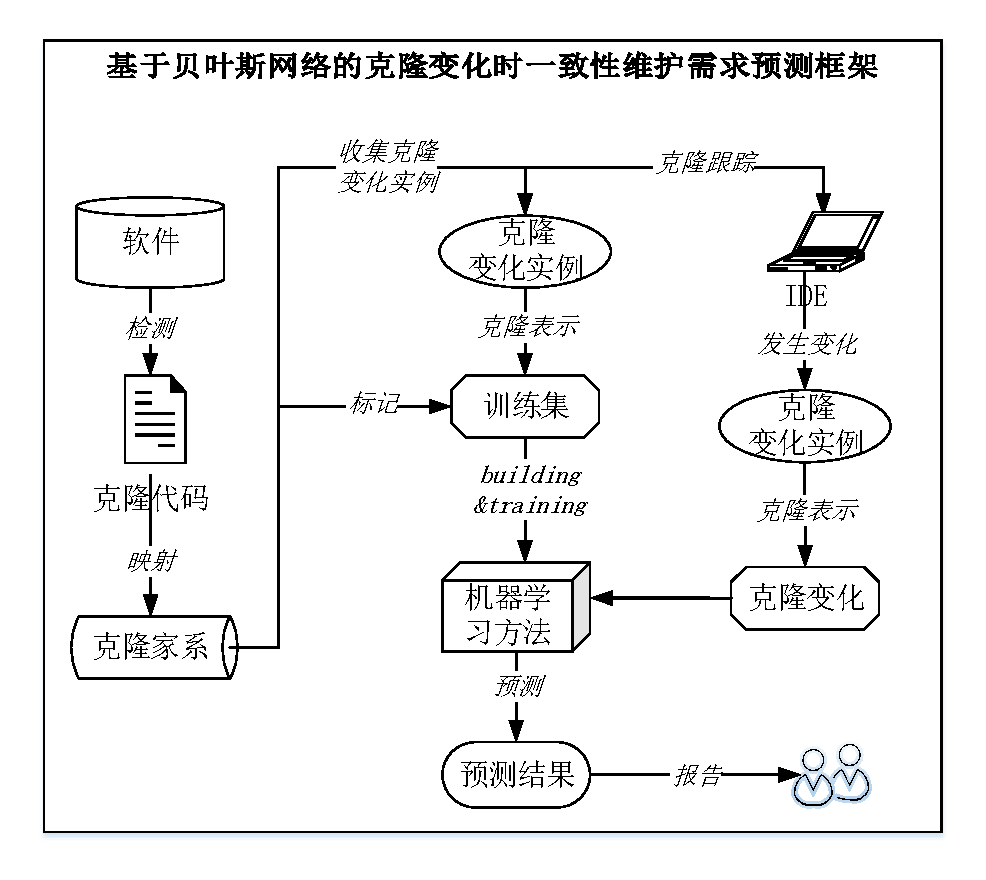
\includegraphics[width = 0.8\textwidth]{framework4.pdf}
\bicaption[framework4]{}{克隆代码修改时一致性维护需求预测框架}
{Fig.$\!$}{The framework for clone changing consistency prediction}
\vspace{-1em}
\end{figure}

在收集阶段中,通过构建系统的克隆家系从软件中收集所有的克隆变化实例。使用NiCad来检测软件版本中的所有克隆,并通过在相邻版本的克隆组之间进行映射来构建克隆家系,用于识别克隆变化实例。在表示阶段中,通过提取属性值表示克隆变化实例,提取了代码属性、上下文属性和历史属性三组属性组,同时,还提取了关于克隆变化的相关信息。在预测阶段中,使用收集到的克隆变化实例训练贝叶斯网络,并在克隆变化时预测克隆一致性维护需求。根据预测结果提醒程序开发人员采取进一步的维护操作。

克隆变化实例有两种不同的预测结果,即满足一致性维护需求和不满足维护需求。对于满足一致性维护需求实例来说,其在将来的演化中可能会引发一致性变化,程序开发人员需要验证克隆组内克隆代码的一致性问题,从而避免此变化所导致的克隆一致性缺陷。对于不满足一致性维护需求实例来说,其在将来的演化中不会引发一致性变化,程序开发人员可以放心的对该克隆代码进行修改,不必考虑克隆一致性问题,更加快速高效地对克隆代码采取维护操作。

\BiSection{克隆变化实例收集}
{Collecting Clone Changing Instance}

收集克隆变化实例的目的在于生成克隆一致性预测的训练集,并将其用于训练机器学习模型。通过构建系统的克隆家系并识别其中的克隆演化模式,可以从软件中收集所有的克隆变化实例。首先,使用NiCad来检测软件版本中的所有克隆。然后,通过在相邻版本的克隆组之间进行映射来构建克隆家系。最后,识别克隆一致性演化模式识别系统中的克隆变化实例。

根据定义~\ref{def-changinginstance}~,本文假定克隆家系$CGE$中发生变化的克隆组为克隆变化实例。因此通过构建克隆家系并识别克隆家系中发生变化的克隆组,可以收集克隆创建实例。

(1)构建克隆家系

首先,下载系统所有版本的源代码,并使用NiCad的默认配置检测检测每一版本的中Type1-3的克隆代码。然后,通过映射所有相邻版本的克隆代码,构建系统中全部克隆家系。为完成版本间的映射,为每个克隆片段生成一个克隆区域描述符 $CRD$\cite{duala2010clone},使用基于CRD的克隆映射算法映射两个连续版本之间的所有克隆片段和克隆组\cite{ci2013new}\cite{ci2013newD}。根据克隆映射结果,构建系统的克隆家系。

(2)识别克隆演化模式和收集克隆变化实例

首先,识别克隆家系中的克隆演化模式。构建克隆家系后,通过对比相邻版本的克隆代码,可以识别克隆家系的克隆演化模式,尤其是一致性变化模式(参考定义~\ref{def-evolutionpattern}~和\ref{def-changingpattern}~)。所识别的克隆演化模式有三个作用:(a)可以用于表示克隆变化实例,本文使用克隆演化模式作为表示克隆变化实例的部分演化属性。因此,克隆演化模式可以用于克隆变化实例表示中。(b)克隆演化模式可以帮助收集克隆变化实例。根据定义~\ref{def-changingchange}~可以识别系统中发生一致性变化的克隆代码和克隆组,从而确定克隆家系中的克隆变化实例。(c)克隆演化模式可以帮助确认克隆一致性维护需求。根据定义~\ref{def-changingrequirement}~,一致性维护需求,可以通过遍历克隆家系$CGE$是否发生了一致性变化模式(定义~\ref{def-changingpattern}~)进行确定。

然后,收集克隆变化实例。在识别克隆家系演化模式,尤其是一致性变化模式后(定义~\ref{def-changingpattern}~),根据定义~\ref{def-changinginstance}通过识别克隆家系中的变化克隆组,便可以收集系统中的克隆变化实例。

(3)标识克隆变化实例的一致性维护需求

在收集所有的克隆变化实例后,还需确认相关实例的一致性需求。根据定义~\ref{def-changingchange}~和~\ref{def-changingrequirement}~,通过遍历克隆变化实例所在的克隆家系$CGE$的演化情况,确定其一致性维护需求。如果克隆变化实例在其演化过程中发生了一致性变化模式(定义~\ref{def-changingpattern}~),则该实例满足一致性维护需求,否则不满足维护需求。

%%%%添加算法

\BiSection{克隆变化实例表示}
{Representing Clone Changing Instance}
\label{lab-changingattribute}

本章使用机器学习中分类方法预测克隆代码变化时的一致性维护需求,并使用软件中既有的克隆变化实例训练不同的机器学习模型。但是,实际的克隆变化实例无法直接应用于机器学习中。因此,本节将提取相应的属性值表示克隆变化实例。将分别提取代码属性、上下文属性和演化属性代表克隆变化实例。其中,克隆变化实例的代码属性和上下文属性与本文第三章中克隆创建实例的属性相似,区别在于克隆变化实例将从克隆组的角度提取相应的属性。同时,本章还从演化的角度提取了演化属性表示克隆变化实例。

\BiSubsection{代码属性}
{Code Attribute}

代码属性从代码自身的角度描述了克隆变化实例中克隆代码特征。代码属性描述了克隆代码的词法、语法和函数调用等信息。代码属性主要包括克隆代码粒度、Halstead属性、结构属性、调用属性等。与第三章中代码属性不同的是,克隆变化实例从克隆组的角度提取相应属性(注意一个克隆变化实体表示一个发生变化的克隆组)。具体的代码属性如下所示:
%类似于\cite{} {Wang2012}中收集的属性。主要区别在于它们的计算:Wang et al。 从两个代码聚集的属性:复制和粘贴代码。这里,我们计算每个属性的平均值,当需要时。因此,我们的属性包括代码行的平均数,参数的平均数,调用调用的平均数。此外,我们有:

\begin{itemize}
\item 
克隆粒度:
在克隆变化实例中,所有克隆片段的数量。
\item 
代码行平均:
在克隆变化实例中,所有克隆片段的平均代码行。
\item 
Halstead属性平均:
在克隆变化实例中,所有克隆片段的Halstead属性平均,有四个基本的度量值,分别为平均操作符种类、平均操作数种类、平均操作符总量和平均操作数总量。
\item
结构属性平均:
在克隆变化实例中,所有克隆片段的结构属性属性平均,包括\verb+if_then+, \verb+if\_else+, \verb+switch+, \verb+while+, \verb+do+, \verb+for+,  \verb+this\_or\_super+等。 
\item 
参数访问数量平均:
在克隆变化实例中,所有克隆片段的参数访问数量统计的平均。
\item  
总函数调用次数平均:
在克隆变化实例中,所有克隆片段的所有函数调用的次数统计。
\item  
本地函数调用次数平均:
在克隆变化实例中,所有克隆片段的调用函数与被复制克隆片段在相同类的调用次数统计平均。
\item  
库函数调用次数平均:
在克隆变化实例中,所有克隆片段的库函数的调用次数统计平均,包括java库函数的调用、eclipse库函数的调用以及第三方包函数的调用。
\item  
其它调用次数平均:
在克隆变化实例中,所有克隆片段中既不是库函数调用、也不是本地函数调用的其它调用次数统计平均,如同项目内其它包函数调用或同包内其它类中的函数调用。
\end{itemize}

%%\begin{itemize}
%%\item Clone Group Size: 
%%The number of code fragments in the clone group.
%% \item Average Code Lines: The average number of code lines for all
%%  clone fragments in clone group.
%%\item Average Number of Halstead: 
%%The average number of Halstead for all clone fragments in clone group. The Halstead includes the number of distinct operators, number of distinct operands, total number of operators, total number of operands.
%% \item Average Number of Parameters: The average number of parameters
%%   for all clone fragments in the clone group.
%%\item Average Number of Important Syntactic Constructs: 
%%For each important syntactic construct (such as \verb+if+, \verb+while+, etc.), we compute the average number of occurrences of the construct for all clone fragments of clone group.
%% \item Average Number of Invocations: The average number of method
%%   invocations for all clone fragments in the clone group, which
%%   includes all invocations, library invocations, local invocations,
%%   and other invocations.
%%\end{itemize}

\BiSubsection{上下文属性}
{Context Attribute}

上下文属性是克隆变化实例中克隆代码之间的关系属性,描述了克隆代码之间的克隆关系信息。上下文属性包括克隆变化实例中的平均代码相似度、克隆分布、所包含克隆代码之间的一些相似度等等。值得注意的是,上下文属性也是从克隆组的角度进行计算,首先计算组内任意两个克隆代码片段的上下文属性,然后将上下文属性加权平均。在本文所使用的克隆组中,大部分的克隆组仅包含两个克隆代码片段,少部分克隆组包含多个克隆片段。具体的上下文属性如下所示:
%上下文该集合包含克隆组中克隆的上下文信息,其中一些类似于Wang等人收集的那些。 在\cite{} {Wang2012}中,主要的区别在于我们计算克隆组中的值,而不仅仅是两个克隆。此外,我们添加了几个属性来描述克隆上下文,例如克隆相似性,参数类型和块信息等。这里是属性列表:

\begin{itemize}
\item
代码相似度平均:
在克隆变化实例中,所有的克隆代码的代码相似度平均,使用和NiCad相同的方式计算\cite{roy2008nicad}。
\item
局部克隆标识:
克隆变化实例中的克隆片段是否在同一个文件中。
\item
文件名相似度平均:
在克隆变化实例中,所有的克隆代码的文件的名相似度平均。假定文件名分别为$M_1$和$M_2$,则文件名相似度为$Sim(M_1,M_2)$,采用编辑距离\cite{levenshtein1966binary}计算(剩余度量中相似度采用相同方法计算)。
\item
文件名相似度变量:
当克隆变化实例中所有克隆片段是局部克隆时,其文件名相似度为1,为非局部克隆时为0。该属性决定文件名相似度是否起效。
\item
方法名相似度平均:
在克隆变化实例中,所有的克隆代码所在方法的方法名字相似度平均。
\item
总参数名相似度平均:
在克隆变化实例中,计算任意两个克隆片段的总参数名相似度,然后对所有的相似度进行加权平均。假定两个克隆代码片段所在方法分别为$M$和$N$,$M$和$N$分别包含$m$和$n$个参数,即$(P_1,P_2,…,P_m)$和$(Q_1,Q_2,…,Q_n)$,则总参数名相似度为$Sum(Sim(P_i,Q_j))$。
\item
最大参数名相似度平均:
在克隆变化实例中,计算任意两个克隆片段的最大参数名相似度,然后对所有的相似度进行加权平均。假定两个克隆代码片段所在方法分别为$M$和$N$,$M$和$N$分别包含$m$和$n$个参数,即$(P_1,P_2,…,P_m)$和$(Q_1,Q_2,…,Q_n)$,该最大参数名相似度为$Max(Sim(P_i,Q_j))$。
\item 
总参数类型相似度平均:
在克隆变化实例中,计算任意两个克隆片段的总参数类型相似度,然后对所有的相似度进行加权平均。假定两个克隆代码片段所在方法分别为$M$和$N$,$M$和$N$分别包含$m$和$n$个参数,其参数类型分别为$(P_1,P_2,…,P_m)$和$(Q_1,Q_2,…,Q_n)$,该参数类型相似度为$Sum(Sim(P_i,Q_j))$。
\item
块信息标识:
在克隆变化实例中,所有的克隆代码的上下文信息是否相同,相同为$1$,反之为$0$。
\end{itemize}

%%\begin{itemize}
%%\item Average Clone Similarity: 
%%The average similarity value between each pair of clones in the clone group. 
%%\item Locality of Clones: 
%%This flag determines if all the clone fragments reside in the same file. 
%%\item Average File Name Similarity : 
%%There are two attributes to average file name similarity: the real similarity and the masked similarity. 
%%The mask similarity is a flag indicating if all clones exist in one file. 
%%In the case when not all the clones are in one file, the real similarity is the average of the similarity measure between the names of the files containing clones. 
%%Here, Levenshtein distance-based similarity \cite{Navarro2001} is used. 
%%\item Average Method Name Similarity: 
%%This is the average of the similarity between the names of the methods in which a clone in the clone group belongs.
%%\item Average Sum of Parameter Similarity (ASPS): 
%%First, we compute the ``sum of parameter similarity'' (SPS) for each clone pair in the group, %%as follows: Let $M_1$ and $M_2$ be the two clones with parameters ($P_1$, $P_2$, $\ldots$, $P_m$) and ($Q_1$, $Q_2$, $\ldots$, $Q_n$) respectively. 
%%We define SPS to be: $\sum_{i=1}^{m}\sum_{j=1}^{n} \mathit{Sim}(P_i,Q_j)$. 
%%The final ASPS is the average of SPS's.
%%\item Average Sum of Parameter Type Similarity (ASPTS): 
%%Similar to ASPS measurement, but applying to parameter type names.
%%\item Average Maximal of Parameter Similarity (AMPS): 
%%For each pair of clones $pc$, we compute the {\em maximal of parameter similarity (MPS)}, which is defined as: $\mathit{Max}(\mathit{Sim}(P_i,Q_j))$, where $1\leq i\leq m$, $1\leq j\leq n$, and $\mathit{Sim}(x, y)$ denotes the similarity between string $x$ and string $y$. 
%%The final AMPS is the average of these MPS's. 
%%\item ``Is-same-block'' Flag:  
%%This flag indicates if all the clones are enclosed within block statements of the same syntax.
%%\end{itemize}

\BiSubsection{演化属性}
{Evolutionary Attribute}

克隆变化实例的最后一组属性是,截止到克隆变化实例发生时,克隆变化实例所在的克隆组的历史演化情况。克隆变化实例的演化属性从克隆家系的角度描述了其所在克隆组的演化情况。演化属性包括,克隆寿命、历史演化模式、上次演化时的演化模式克以及克隆组的历史变化等。(具体的演化属性如下所示:

\begin{itemize}
\item 
变化实例寿命:
截止到克隆变化实例发生时,变化实例所在的克隆组的寿命,即在系统中存在的版本数量。
\item 
历史演化模式统计:
截止到克隆变化实例发生时,变化实例所在的克隆组的历史演化模式统计,包括7种克隆演化模式。
\item 
当前演化模式:
截止到克隆变化实例发生时,变化实例所在的克隆组的当前所具有的演化模式,包括7种克隆演化模式。
\item 
历史变化统计:
截止到克隆变化实例发生时,变化实例所在的克隆组的所有的历史变化统计。计算方式如下: 使用克隆变化实例所在克隆组的代码属性变化进行计算。假设克隆变化实例所在的克隆组$CG_j$存在于软件版本$j$中,统计该克隆组从开始出现到此次变化发生时的每一次代码属性的变化。针对每一个代码属性,相邻两个版本之间的代码属性每增加一次,记录为一次正向变化,反之,记录为一次逆向变化。最后,统计每一个代码属性的所有变化,极为历史变化统计。
\end{itemize}

%\begin{itemize}
%\item Clone Group Age: 
%The number of versions the clone group has existed in this repository until now.
%\item Number of Clone Patterns: 
%The number of clone patterns which this clone group experiences until now since its inception. 
%For each clone pattern, we determine the number of occurrences of this pattern in the clone group's history.
%\item Current Pattern: 
%The clone pattern of this clone group, as derived from its change (or unchanged) from the previous version (as formally specified in Definition~\ref{defn-2}.)
%\item Summaries of Clone Changes: 
%The number of changes of this clone group since its inception until the current version.
%For each important code syntax (as specified in the set of code attributes), we capture two pieces of information: We summarize the number of times in the clone genealogy (till the present version) that the syntax experiences an increase (and decrease) in its value from one version to the next immediate version. 
%For instance, suppose that from the clone genealogy, we discover that a clone group originates in version $i$, and evolves till current version $j$ (where $j > i$). 
%We then compare the {\em changes} in the average number of \verb+if+ statements (one of the clone attributes) between two successive versions: versions $i$ and $i+1$, $\cdots$, versions  $j-1$ and $j$. 
%This returns to us a series containing positive and negative numbers.
%We then record the total number of positives and negatives, forming two summaries associated with \verb+if+statements.
%\end{itemize}


最后,对于克隆变化实例,本节还收集了与此次变化相关的一些变化信息,用于描述克隆变化本身。计算方式和演化属性中的“历史变化统计”属性中的计算方法一样。

\begin {itemize}
\item
克隆变化信息:
此次克隆变化发生时,克隆变化实例的变化信息统计。演化属性中的“历史变化统计”属性。
\end {itemize}

%\begin{itemize}
%\item Current Clone Change: 
%The change of this clone group from the current version to the immediate next.  
%We capture this change for each important syntactic construct.
%\end{itemize}

%%%%%\BiSubsection{机器学习方法}
%%%%%{The Employed Machine Learning Methods}
%%%%%%{The Brief Introduction for Machine Learning Methods}
%%%%%
%%%%%在本章的实证研究中,为解决本文所提出的研究问题,使用了五种不同的机器学习方法,即:贝叶斯网络方法(Bayesian Network,简称为BayesNet)\cite{friedman1997bayesian}、朴素贝叶斯方法(Native Bayesian,本文简称为Native)\cite{john1995estimating},支持向量机方法(Support Vector Machine,简称为SVM)\cite{platt199912} 、K近邻方法(K-Nearest Neighbors,简称为KNN) \cite{aha1991instance}和决策树方法(Decision Tree,本文简称为Tree)\cite{quinlan2014c4}。
%%%%%
%%%%%(1)贝叶斯网络方法\\
%%%%%贝叶斯网络是一个是一种概率图型,使用已经观察到的事件来预测将来可能发生的事件\cite{friedman1997bayesian}。关于贝叶斯网络的信息可以参考本文第三章~\ref{lab-bayes}~节贝叶斯网络。
%%%%%
%%%%%(2)朴素贝叶斯方法\\
%%%%%朴素贝叶斯方法和贝叶斯网络类似,是运用贝叶斯定理为基础的简单概率分类器。但与贝叶斯网络不同的是,朴素贝叶斯方法的特征之间是强(朴素)独立的,因此称为朴素贝叶斯,即假定样本每个特征与其他特征都不相关。 
%%%%%
%%%%%(3)支持向量机方法\\
%%%%%支持向量机是另一种常见的机器学习方法,可以应用在分类与回归问题中。SVM模型将实例表示为空间中的点,并且试图构造一个超平面将不同类的实例(点)间隔开。更正式地来说,支持向量机在高维或无限维空间中构造超平面或超平面集合,可以用于分类问题中。直观来说,分类边界距离最近的训练数据点越远越好,因为这样可以缩小分类器的泛化误差。
%%%%%
%%%%%以本文的克隆一致性需求分类为例,每一个克隆代码实例会抽象称为高维空间中的一个“点”,空间维数等同于所提取的属性数量。在使用SVM分类克隆实例时,将构造一个超平面分割开两种类别的克隆代码实例。
%%%%%
%%%%%(4)K近邻方法\\
%%%%%KNN方法是一种用于分类和回归的非参数统计方法。KNN是一种基于实例的学习方法,是局部近似和将所有计算推迟到分类之后的惰性学习。KNN会推迟对训练数据的建模,直到需要分类样本时才进行。在KNN分类中,输出是一个分类族群。一个实例的分类是由其邻居的“多数表决”确定的,K个最近邻居(k为正整数,通常较小)中最常见的分类决定了赋予该对象的类别。若k = 1,则该对象的类别直接由最近的一个节点赋予。邻居都取自一组已经正确分类(在回归的情况下,指属性值正确)的对象。
%%%%%
%%%%%以本文克隆一致性预测为例,每一个克隆代码实例是KNN中的一个实例。在进行预测时,被预测的克隆实例的类别,将会有其最近的K个邻居进行表决,从而确定其一致性维护需求。
%%%%%
%%%%%(5)决策树方法\\
%%%%%机器学习中另一个常见的分类方法是决策树。决策树是一种简单但是广泛使用的分类器。通过训练数据构建决策树,可以高效的对未知的数据进行分类。决策树代表的是属性值与对象类别之间的一种映射关系。树中每个节点表示某个属性,而每个分叉路径则代表的某个可能的权重,而每个叶结点则对应从根节点到该叶节点所经历的路径所表示的对象的类别。决策树仅有单一输出,若欲有复数输出,可以建立独立的决策树以处理不同输出。
%%%%%
%%%%% 以克隆一致性需求预测为例,克隆实例所提取的属性即是决策树中的属性,最后的克隆一致性维护需求则是对象的类别。
%%%%%%决策树(decision tree)是一个树结构(可以是二叉树或非二叉树)。其每个非叶节点表示一个特征属性上的测试,每个分支代表这个特征属性在某个值域上的输出,而每个叶节点存放一个类别。使用决策树进行决策的过程就是从根节点开始,测试待分类项中相应的特征属性,并按照其值选择输出分支,直到到达叶子节点,将叶子节点存放的类别作为决策结果。

\BiSection {克隆代码变化时一致性需求预测}
{Predicting Clone Changing Consistency-Requirement} 

本章将克隆代码变化时的一致性维护需求问题,转化成了克隆变化实例的分类问题,即给定一个克隆变化实例,判别其是否满足克隆变化时的一致性维护需求。本节使用五种机器学习方法作为机器学习模型,并使用其预测克隆一致性维护需求,即贝叶斯网络方法、朴素贝叶斯方法、支持向量机方法、K近邻方法和决策树方法(方法简介可参考本文第~\ref{lab-machine}~节机器学习方法简介)。

与第三章类似,本章也没有对机器学习方法进行改进,模型的构建和训练通过调用现有机器学习工具包WEKA完成。对于每个软件系统,首先,通过收集克隆变化实例并提取相应的属性,用于构建模型训练所需的数据集。然后,调用WEKA中的机器学习方法构建和训练克隆一致性预测模型。

根据定义~\ref{def-changingrequirement}~,克隆变化实例有两种不同的状态:需要一致性维护和不需要一致性维护。因此在进行一致性维护需求预测时,克隆变化实例也具有两种不同的预测结果:

\begin{itemize}
\item 
需要一致性维护:
若克隆变化实例的预测结果为“需要”,软件开发人员需要检测克隆变化实例所在的克隆组的一致性问题,考虑一致地修改组内其它的克隆代码。因为,该克隆变化实例,在未来演化的过程中可能会引发一致性变化,遗忘这种变化会向系统中引入缺陷,从而降低软件质量。
\item
不需要一致性维护:
若克隆创建实例的预测结果为“不需要”,软件开发人员可以自由的修改克隆变化实例所在克隆组的克隆片段。因为,该克隆变化实例,在未来演化的过程中不会引发一致性变化,也不会导致一致性缺陷。
\end{itemize}

在使用已训练好的模型进行预测时,可以与软件开发过程相结合,将该模型嵌入到软件开发环境中,帮助程序开发人员实现边开发边预测克隆变化实例的一致性维护需求。首先,在软件开发环境中需监测程序员对克隆代码的修改,识别由此产生的克隆变化实例。然后,根据上文描述的代码、上下文和演化属性,提取相应的特征表示该克隆变化实例。最后,使用训练好的预测器预测该克隆变化实例的一致性维护需求,根据预测结果提醒程序开发人员采取进一步的操作。

%%%\BiSection{算法描述}
%%%{algorithm description}

\BiSection{实验结果与分析}
{Experimental Results and Analysis}

%本节给出本章的实验结果与分析,首先简单介绍了实验所使用的实验系统和评估方法,然后详细给出每个实验的结果与分析。

\BiSubsection{实验系统与实验设置}
{Experimental Projects and Methodology}

为评估本章方法,本章选取了四个开源软件进行实验。四个实验系统的克隆变化实例统计情况如表~\ref{changesta}~所示。具体来说,第3列和第4列分别给出了不需要一致性维护和需要一致性维护的克隆变化实例的数量和比例。不需要一致性维护的克隆变化实例,该克隆变化不会使其所在的克隆组在未来演化中发生一致性变化,因此程序人员无需关注其克隆组的一致性问题。需要一致性维护的克隆变化实例,该克隆变化可能使其所在克隆组在未来演化过程中发生一致性变化,而遗忘这种变化会导致克隆缺陷,从而降低软件质量。

从表中~\ref{changesta}~可以得出两个发现。第一,每个实验系统中都有数百到上千的克隆变化实例,数量从159到1040个,其中项目{jEdit}是含有最少的克隆变化实例。第二,在这些变化实例中,需要一致性维护的克隆实例比例占相当大的一部分,其比例为33\%到74\%。其中,ArgoUML中大部分的克隆变化实例不需要一致性维护。jEdit和jFreeChart需要和不需要一致性维护的克隆变化实例数量相差不大。而Tuxguitar中的克隆变化实例大部分都需要一致性维护。尽管需要一致性维护的克隆变化实例远远少于克隆创建实例(表~\ref{copysta}~),但是仍在存在数百个需要一致性维护的实例,同时克隆变化实例的危害也更大。因为对克隆变化实例来讲,需要一致性维护的克隆实例比例更大,也更容易导致缺陷。

\begin{table}[htbp]
\bicaption[changesta]{}{实验系统的克隆变化实例信息统计}
{Table$\!$}{The statistics for clone creating instances in four projects}
\vspace{0.5em}
\centering
\wuhao
\begin{tabular}{cccc}
\toprule[1.5pt]
~\multirow{2}{*}{实验系统}& \multicolumn{2}{c}{克隆变化实例的数量(比例)} & \multirow{2}{*}{总数}\\ 
 \cline{2-3}
~&{不需要维护} &{需要维护} & ~\\
\midrule[1pt]
ArgoUML&288(67.45\%)&139(32.55\%)&427\\
jEdit&78(49.06\%)&81(50.94\%)&159\\
jFreeChart&452(43.46\%)&588(56.54\%)&1040\\
Tuxguitar&91(25.71\%)&263(74.29\%)&354\\
\bottomrule[1.5pt]
\end{tabular}
\end{table}

表~\ref{changeclonenumbersta}~给出了四个实验系统中克隆变化实例所包含的克隆代码的数量的统计信息。表中最后一列显示了克隆代码数量为2。因此,系统中虽然有大量的克隆代码,但是变化实例所包含的克隆数量并不是很多。同时,ArgoUML和 jFreeChart系统中存在少量的超大克隆组,从而导致了平均值和标准差较大。

\begin{table}[htbp]
\bicaption[changeclonenumbersta]{}{克隆变化实例的克隆代码数量信息统计}
{Table$\!$}{Statistics of the size of clone change instances}
\vspace{0.5em}
\centering
\wuhao
\begin{tabular}{ccccc}
\toprule[1.5pt]
{实验系统}&{数量}&{Mean}&{Standard Deviation}&{Median}\\ 
\midrule[1pt]
ArgoUML&427&7.593&	26.224&2\\
jEdit&159&	2.465&	0.913&2\\ 
jFreeChart&1040&	7.853&	26.924&2\\
Tuxguitar&354&	3.404	&3.452&2\\ 
\bottomrule[1.5pt]
\end{tabular}
\end{table}

%%%%\begin{table}[htbp]
%%%%\bicaption[changeclonenumbersta]{}{克隆变化实例的克隆代码数量信息统计}
%%%%{Table$\!$}{Statistics of the size of clone change instances}
%%%%\vspace{0.5em}
%%%%\centering
%%%%\wuhao
%%%%\begin{tabular}{ccccc}
%%%%\toprule[1.5pt]
%%%%\textbf{Project}&\textbf{Total}&\textbf{Mean}&\textbf{Standard Deviation}&\textbf{Median}\\ 
%%%%\midrule[1pt]
%%%%ArgoUML&427&7.5.9271&	26.22377&2\\
%%%%jEdit&159&	2.46541&	0.9125&2\\ 
%%%%jFreeChart&1040&	7.85288&	26.92378&2\\
%%%%Tuxguitar&354&	3.40395	&3.45232&2\\ 
%%%%\bottomrule[1.5pt]
%%%%\end{tabular}
%%%%\end{table}

表~\ref{changelifesta}描述了克隆变化实例发生变化时的寿命统计信息。如前所述,克隆变化实例寿命年龄是自其所在的克隆组在发生变化时,所经历的所有软件版本的数量(从$0$开始计算)。从表中可以看出,克隆变化实例的寿命普遍偏小。考虑到克隆变化实例的本质,即被开发人员修改的克隆代码。克隆代码变化可能会较早的出现,因此需要尽可能早地执行克隆的一致性要求,从而避免引入过多的克隆一致性缺陷。

\begin{table}[htbp]
\bicaption[changelifesta]{}{克隆变化实例寿命信息统计}
{Table$\!$}{Statistics for clone life of clone change instances}
\vspace{0.5em}
\centering
\wuhao
\begin{tabular}{ccccc}
\toprule[1.5pt]
{实验系统}&{数量}&{Mean}&{Standard Deviation}&{Median}\\ 
\midrule[1pt]
ArgoUML&427&2.094&2.331&1\\ 
jEdit&159&4.484&3.644&3\\ 
jFreeChart&1040&4.935&4.995&3\\ 
Tuxguitar&354&1.557&1.503&1\\ 
\bottomrule[1.5pt]
\end{tabular}
\end{table}

%%%%\begin{table}[htbp]
%%%%\bicaption[changelifesta]{}{克隆变化实例寿命信息统计}
%%%%{Table$\!$}{Statistics for clone life of clone change instances}
%%%%\vspace{0.5em}
%%%%\centering
%%%%\wuhao
%%%%\begin{tabular}{ccccc}
%%%%\toprule[1.5pt]
%%%%{实验系统}&{数量}&\textbf{Mean}&\textbf{Standard Deviation}&\textbf{Median}\\ 
%%%%\midrule[1pt]
%%%%ArgoUML&427&2.09368&2.33078&1\\ 
%%%%jEdit&159&4.48428&3.64371&3\\ 
%%%%jFreeChart&1040&4.93462&4.99543&3\\ 
%%%%Tuxguitar&354&1.5565&1.50294&1\\ 
%%%%\bottomrule[1.5pt]
%%%%\end{tabular}
%%%%\end{table}

本节首先使用贝叶斯网络模型预测克隆创建实例的一致性,预测时贝叶斯网络会计算克隆变化实例的概率值,表示该实例需要一致性维护需求的概率(在0~1之间,数值接近于1表示需要一致性维护,接近于0表示不需要一致性维护)。然后,在其它五种不同的机器学习方法上进行了实验,对比选择最优的机器学习方法。

为全面评估本文方法,将实验进一步的划分为全属性实验、属性组实验:

\begin{itemize}
\item
全属性实验:
使用本章提取的所有属性对实验系统进行分析,评估本文方法的预测能力。
\item
属性组实验:
分别使用两组不同的属性组对实验系统进行分析,评估所提取的属性组对预测能力的影响。
%%%\item
%%%交叉验证实验:使用其它系统数据作为训练集训练模型,并使用该模型在新系统上进行实验分析,从而探索模型在应用到新系统的预测能力。
\end{itemize}

%我们在具有Intel(R)Core(TM)i5-4210M CPU @ 2.60GHz和8G RAM的桌面上运行我们的实验。每个实验花费不到一分钟的模型构建,交叉验证少于5分钟。大多数实验时间花费在数据准备,包括家谱建构和克隆变化实例收集,其范围在5至30分钟之间。然而,我们注意到,在实践中,克隆系谱构建和变更实例收集将逐步执行,随着软件发展到新版本。因此,数据准备的开销将不是实际问题。

\BiSubsection{贝叶斯网络实验}
{Clone Changing Consistency-Requirement Experiment}
\label{ref-changingbayesianmetrics}

本节使用使用开源软件工具WEKA训练和预测贝叶斯网络。在构建贝叶斯网络时,使用K2搜索算法建立网络结构,并设置贝叶斯网络最大父节点个数为4,使用{\em  SimpleEstimator}来估计贝叶斯网络的条件概率表。在实验时,采用十倍交叉验证(10-folds Cross-Validity)的方式,将克隆变化实例的数据集划分为训练集和测试集,使用训练集训练贝叶斯网络生成预测模型,然后使用测试集评估贝叶斯网络的预测能力。

针对不同的克隆变化实例,与第三章类似,也设置了不同的阈值进行实验分析。对于需要一致性维护的实例,其贝叶斯网络预测值较大(接近于1),选取阈值为0.5、0.6、0.7、0.8和0.9,当预测值大于等于该阈值认定该实例需要一致性维护。对于不需要一致性维护的实例,其预测值较小(接近于0),选取阈值为0.01、0.05、0.10、0.15和0.20,当预测值小于等于给定阈值时认定该实例不需要一致性维护。

\BiSubsubsection{一致性维护需求实验}
{Clone Changing Consistency Experiment}

在本节中,对需要一致性维护的克隆变化实例进行评估。关注需要一致性维护的克隆变化实例,由于该变化可能会导致其所在的克隆组在演化过程中的一致性变化模式,因此需要警告程序开发人员检查克隆组的一致性问题,避免克隆一致性缺陷。实验采用三个度量对方法进行评估,即警告率、精确率和召回率,描述如下:

\begin{itemize}
\item 
警告率(Warning Rate):指所警告的需要一致性维护的克隆变化实例,即预测为需要一致性维护的实例与系统中全部实例的比值。这些克隆变化实例可能会导致一致性缺陷问题,需要确保克隆组的一致性。

\item 
精确率(Precision):指警告为需要一致性维护的克隆变化实例的精确率,即在所预测为需要一致性维护的变化实例中,正确预测的实例与全部警告实例的比值。

\item 
召回率(Recall):指所警告的需要一致性维护的克隆变化实例的召回率,即预测为需要一致性维护的实例与系统中的真实的需要一致性维护实例的比值。
\end{itemize}

%%%%\BiSubsubsection{全属性组实验}
%%%%{Effectiveness Experiment}

(1)全属性组实验

全属性实验使用本章提取的全部属性组在四个实验系统上进行评估,实验结果如表~\ref{changeallmeeting}所示。

所创建的模型在预测jFreeChart和Tuxguitar的一致性需求时,预测结果显示非常有效,其中预测的准确度和召回率在80\%左右。同时,jEdit系统的预测效果虽然不如上面两个系统好,但是也相当不错。原因可能是因为jEdit系统的克隆变化实例规模较小,没有对模型实现较好的预测,但这需要进一步研究。尽管ArgoUML的预测效果不如其它系统的预测效果,但其精确率仍然可以达到65\%左右,且召回率在45\%左右。最后,对于四个实验系统,本文所构建的模型均具有有十分合理的警告率,警告率十分接近于满足一致性维护需求的克隆变化实例的比例(如表~\ref {changesta}~中所示)。

虽然阈值的变化可以影响预测的精确率和召回率,但影响并不是十分的剧烈,对召回率的影响要比精确率的影响更大。这意味着本文所创建的模型可以提供相当准确的预测效果,但仍需进一步增强预测模型的召回能力。因此,开发人员可以较为自信地依赖于本文的预测结果,但需要其它方法来避免那些预测为不需要一致性维护的错误实例,从而帮助提高模型的预测效果。一个简单简单有效的改进方法是在克隆创建时尽量避免避免那些可能会引发一致性维护的克隆实例,具体细节可参考本文第三章提出的克隆创建时克隆一致性预测方法。

\begin{table}[htbp]
\bicaption[changeallmeeting]{}{四个实验系统全属性的实验效果}
{Table$\!$}{The effectiveness for all attribute sets on four projects}
\vspace{0.5em}
\centering
\wuhao
\begin{tabular}{ccccc}
\toprule[1.5pt]
{实验系统}&{阈值}&{警告率(\%)}&{精确率(\%)}&{召回率(\%)}\\
\midrule[1pt]
 \multirow{5}{*}{ArgoUML}
&0.9&	20.14&	69.77&	43.17\\
&0.8&	21.31&	68.13&	44.60\\
&0.7&	24.12&	65.05&	48.20\\
&0.6&	24.59&	63.81&	48.20\\
&0.5&	25.29&	62.04&	48.20\\
\hline
\multirow{5}{*}{jEdit}
&0.9&	43.40&	73.91&	62.96\\
&0.8&	47.17&	70.67&	65.43\\
&0.7&	49.06&	70.51&	67.90\\
&0.6&	50.31&	70.00&	69.14\\
&0.5&	50.94&	69.14&	69.14\\
\hline
\multirow{5}{*}{jFreeChart}
&0.9&	52.50&	82.05&	76.19\\
&0.8&	55.19&	81.36&	79.42\\
&0.7&	56.83&	80.71&	81.12\\
&0.6&	58.65&	80.33&	83.33\\
&0.5&	60.10&	79.68&	84.69\\
\hline
\multirow{5}{*}{Tuxguitar}
&0.9	&76.55&   80.44&	82.89\\
&0.8	&78.53&	80.22&	84.79\\
&0.7	&80.51&	80.00&	86.69\\
&0.6	&81.64&	79.24&	87.07\\
&0.5    &83.33&	79.32&	88.97\\
\bottomrule[1.5pt]
\end{tabular}
\end{table}

%%%\BiSubsubsection{属性组实验}
%%%{Attribute Set Experiment}

(2)属性组实验

本章提取的了三组属性表示克隆变化实例,从不同的角度描述了变化实例的特征。为评估不同的属性组对预测效果的作用,本节进行了属性组实验。表~\ref{changesetmeeting}~中给出了属性组的评估实验结果。其中,分别给出了使用全部属性和删除每一组属性后的实验结果,即“全部属性”、“无代码属性”、“无上下文属性”和“无演化属性”。

从表中可以看出,属性组对预测结果的影响并无一致性结论。但是,代码属性和上下文属性与全属性组对比表明,这两组属性对预测的召回率有显著影响。但是,无演化组属性的实验结果表明其对实验结果的影响没有预想的那么大。尽管如此,这些属性组依然对预测效果有影响,但需要进一步的研究去寻找这种差异背后的真正原因。

此外,本章还对所选用的属性组进行了属性选择实验,使用WEKA提供的功能选取了最佳属性集。然而,通过比对全属性组的实验结果,发现发现全属性组实验结果要优于最佳属性组实验结果,所采用的属性具有积极的意义。虽然一些属性组可能对实验结果没有显着的影响,但是其也不具有消极的影响。本章建议在进行一致性预测时,需要保留全部属性组,因为在应用到其它系统是可能会起到积极的作用。

\begin{sidewaystable} 
\bicaption[changesetmeeting]{}{在四个实验系统上属性组实验效果}
{Table$\!$}{The effectiveness for attribute set on four projects}
\vspace{0.5em}
\centering
\wuhao
\begin{tabular}{cccccccccccccc}
\toprule[1.5pt]
\multirow{2}{*}{实验系统}&\multirow{2}{*}{阈值}&\multicolumn{3}{c}{全部属性(\%)}&\multicolumn{3}{c}{无代码属性(\%)}&\multicolumn{3}{c}{无上下文属性(\%)}&\multicolumn{3}{c}{无演化属性(\%)}\\
\cline{3-14}
&&{警告率}&{精确率}&{召回率}&{警告率}&{精确率}&{召回率}&{警告率}&{精确率}&{召回率}&{警告率}&{精确率}&{召回率}\\
\midrule[1pt]
\multirow{5}{*}{ArgoUML}
&0.9&20.14&	69.77&	43.17&14.29&	73.77&	32.37&17.56&	72.00&	38.85&21.78&	69.89&	46.76\\
&0.8&	21.31&	68.13&	44.60&	20.37&	70.11&	43.88&	19.91&	69.41&	42.45&	24.12&	66.02&	48.92\\
&0.7&	24.12&	65.05&	48.20&	23.89&	65.69&	48.20&	21.78&	64.52&	43.17&	26.00&	63.96&	51.08\\
&0.6&	24.59&	63.81&	48.20&	25.76&	63.64&	50.36&	24.12&	63.11&	46.76&	28.10&	60.00&	51.80\\
&0.5&	25.29&	62.04&	48.20&	29.27&	61.60&	55.40&	26.00&	59.46&	47.48&	29.51&	60.32&	54.68\\
\hline
\multirow{5}{*}{jEdit}
&0.9&	43.40&	73.91&	62.96&	38.99&	75.81&	58.02&	40.88&	75.38&	60.49&	44.03&	71.43&	61.73\\
&0.8&	47.17&	70.67&	65.43&	43.40&	72.46&	61.73&	46.54&	70.27&	64.20&	47.80&	69.74&	65.43\\
&0.7&	49.06&	70.51&	67.90&	47.17&	70.67&	65.43&	47.80&	71.05&	66.67&	49.69&	68.35&	66.67\\
&0.6&	50.31&	70.00&	69.14&	48.43&	71.43&	67.90&	47.80&	71.05&	66.67&	51.57&	65.85&	66.67\\
&0.5&	50.94&	69.14&	69.14&	53.46&	69.41&	72.84&	50.94&	67.90&	67.90&	52.83&	65.48&	67.90\\
\hline
\multirow{5}{*}{jFreeChart}
&0.9&	52.50&	82.05&	76.19&	44.42&	84.63&	66.50&	51.06&	81.92&	73.98&	50.19&	81.42&	72.28\\
&0.8&	55.19&	81.36&	79.42&	49.42&	82.10&	71.77&	54.13&	80.99&	77.55&	53.56&	80.07&	75.85\\
&0.7&	56.83&	80.71&	81.12&	53.17&	80.83&	76.02&	56.92&	79.39&	79.93&	56.06&	78.39&	77.72\\
&0.6&	58.65&	80.33&	83.33&	55.10&	80.10&	78.06&	59.33&	78.12&	81.97&	57.50&	77.93&	79.25\\
&0.5&	60.10&	79.68&	84.69&	57.79&	78.20&	79.93&	60.48&	78.06&	83.50&	59.13&	77.56&	81.12\\
\hline
\multirow{5}{*}{Tuxguitar}
&0.9&	76.55&	80.44&	82.89&	68.64&	79.01&	73.00&	75.14&	78.57&	79.47&	71.75&	80.71&	77.95\\
&0.8&	78.53&	80.22&	84.79&	74.01&	79.01&	78.71&	78.53&	78.42&	82.89&	74.01&	80.92&	80.61\\
&0.7&	80.51&	80.00&	86.69&	78.25&	78.34&	82.51&	80.79&	77.97&	84.79&	76.55&	80.81&	83.27\\
&0.6&	81.64&	79.24&	87.07&	79.94&	78.09&	84.03&	82.20&	77.32&	85.55&	78.53&	80.94&	85.55\\
&0.5&	83.33&	79.32&	88.97&	83.33&	77.63&	87.07&	84.18&	76.85&	87.07&	79.66&	80.50&      86.31\\
\bottomrule[1.5pt]
\end{tabular}
\end{sidewaystable}

\BiSubsubsection{一致性维护自由实验}
{Clone Changing Consistency Free Experiment}

本节实验对不需要一致性维护的克隆变化实例进行预测评估。将关注不需要一致性维护的克隆实例,从而让程序开发人员可以更加自由的修改克隆代码,而不需要考虑克隆变化所引发的一致性维护问题,可以更加快速有效的开发系统。此实验使用三个度量评估预测效果,分别为:推荐率、精确率和召回率,如下所示:

\begin{itemize}
\item 
推荐率(Recommendation Rate):
指的是所推荐的不需要一致性维护的克隆变化实例与所有实例的比例,即预测为不需要一致性维护的克隆变化实例与系统中全部变化实例的比值。
\item 
精确率(Precision):
指所预测的不需要一致性维护克隆变化实例的精确率,即在预测为不需要一致性维护的克隆变化实例中,正确预测的实例与所预测实例的比值。
\item  
召回率(Recall):
指所推荐的不需要一致性维护的克隆变化实例的查全率,即预测为不需要一致性维护的变化实例,与系统中的不需要一致性维护的实例的比值。
\end{itemize}

%%\BiSubsubsection{全属性组实验}
%%{Effectiveness Experiment}
(1)全属性实验

全属性实验使用全部属性在四个实验系统上进行评估,实验结果如表~\ref{changeallfree}~所示。

由表中可以看出,本文方法在预测不需要一致性维护的克隆变化实例时,在四个系统上均取得了不错的预测效果。其中,在系统ArgoUML和 jFreeChart取得了较好的效果,精确率在80\%左右,并且召回率在70\%左右。在系统 jEdit的预测效果尽管没有上面两个系统的预测效果好,但也具有不错的预测效果。然而不幸的是,本文的方法在系统Tuxguitar上预测效果不够理想,精确率在50\%左右,召回率更低。可能是由于Tuxguitar的不满足一致性维护需求的克隆变化实例太少,没有对预测模型训练完全,但是仍需进一步的研究确认。同时,本文所构建的模型在四个系统上都具有十分合理的推荐率,推荐率和系统本身的不需要一致性维护的克隆变化的比例相差不大(如表~\ref{changesta}~中所列)。

不同的阈值会影响到精确率和召回率,但是阈值对于召回率的影响要大于大于精确率的影响。这意味着本文所构建的模型可以提高比较稳定的预测效果(精确率差不大),但系统的召回率仍需要进一步的提升。简而言之,本文的方法所构建的预测模型可以对不需要一致性维护的克隆变化实例提供一个相对稳定的预测,并且具有相当好的准确度和召回率,软件开发人员可以据此对克隆变化实例进行有效的预测。


\begin{table}[htbp]
\bicaption[changeallfree]{}{四个实验系统的全属性组实验效果}
{Table$\!$}{The effectiveness for all attribute on four projects}
\vspace{0.5em}
\centering
\wuhao
\begin{tabular}{ccccc}
\toprule[1.5pt]
{系统}&{阈值}&{推荐率(\%)}&{精确率(\%)}&{召回率(\%)}\\
\midrule[1pt]
\multirow{5}{*}{ArgoUML}
&0.01&	51.99&	83.33&	64.24\\
&0.05&	60.42&	82.95&	74.31\\
&0.1&	63.93&	81.32&	77.08\\
&0.15&	65.81&	80.43&	78.47\\
&0.2&	67.45&	80.21&	80.21\\
\hline
\multirow{5}{*}{jEdit}
&0.01&	20.13&	84.38&	34.62\\
&0.05&	30.19&	79.17&	48.72\\
&0.1&	33.96&	74.07&	51.28\\
&0.15&	38.36&	70.49&	55.13\\
&0.2&	39.62&	69.84&	56.41\\
\hline
\multirow{5}{*}{jFreeChart}
&0.01&	28.65&	84.56&	55.75\\
&0.05&	32.50&	83.73&	62.61\\
&0.1&	34.23&	82.02&	64.60\\
&0.15&	35.58&	80.81&	66.15\\
&0.2&	36.06&	80.53&	66.81\\
\hline
\multirow{5}{*}{Tuxguitar}
&0.01&	7.91&	53.57&	16.48\\
&0.05&	9.32&	57.58&	20.88\\
&0.1&	9.89&	54.29&	20.88\\
&0.15&	12.15&	48.84&	23.08\\
&0.2&	13.28&	48.94&	25.27\\
\bottomrule[1.5pt]
\end{tabular}
\end{table}



%%%\BiSubsubsection{属性组实验}
%%%{Attribute Set Experiment}
(2)属性组实验

同样,对不需要一致性维护的克隆变化实例,本章同样进行了属性组实验,以评估不同的属性组对预测效果的影响。实验结果如表~\ref{changesetfree}~所示,其中,分别给出了使用全部属性和删除每一组属性后的实验结果,即“全部属性”、“无代码属性”、“无上下文属性”和“无演化属性”。

从表中可以看出,属性组对“一致性维护自由”实验的预测结果的影响并无一致性结论。但是,代码属性和上下文属性与全属性组对比表明,这两组属性对预测的召回率有显著影响。但是,无演化组属性的实验结果表明其对实验结果的影响没有预想的那么大。尽管如此,这些属性组依然对预测效果有影响,但需要进一步的研究去寻找这种差异背后的真正原因。

此外,本文还对所选用的属性组进行了属性选择实验,使用WEKA提供的功能选取了最佳属性集。然而,通过比对全属性组的实验结果,发现发现全属性组实验结果要好于最佳属性子集的实验结果,因此,所采用的属性具有积极的意义。虽然一些属性组可能对实验结果没有显着的影响,但是其也不具有消极的影响。

尽管一些属性组可能对实验结果没有极为重要的贡献,但是属性组同样也没有产生消极的影响。因此,本文建议将所有属性保留在构建预测模型中,因为某些属性可能对一些未经实验验证的系统具有重要且积极的影响。

\begin{sidewaystable} 
\bicaption[changesetfree]{}{在四个实验系统上属性组实验效果}
{Table$\!$}{The effectiveness for attribute set on four projects}
\vspace{0.5em}
\centering
\wuhao
\begin{tabular}{cccccccccccccc}
\toprule[1.5pt]
\multirow{2}{*}{实验系统}&\multirow{2}{*}{阈值}&\multicolumn{3}{c}{全部属性(\%)}&\multicolumn{3}{c}{无代码属性(\%)}&\multicolumn{3}{c}{无上下文属性(\%)}&\multicolumn{3}{c}{无演化属性(\%)}\\
\cline{3-14}
&&{警告率}&{精确率}&{召回率}&{警告率}&{精确率}&{召回率}&{警告率}&{精确率}&{召回率}&{警告率}&{精确率}&{召回率}\\
\midrule[1pt]
\multirow{5}{*}{ArgoUML}
&0.01&	51.99&	83.33&	64.24&	36.77&	89.17&	48.61&	48.01&	83.41&	59.38&	44.03&	85.64&	55.90\\
&0.05&	60.42&	82.95&	74.31&	49.18&	85.71&	62.50&	59.48&	79.92&	70.49&	51.99&	84.23&	64.93\\
&0.1&	63.93&	81.32&	77.08&	56.67&	83.06&	69.79&	63.00&	79.18&	73.96&	58.31&	83.53&	72.22\\
&0.15&	65.81&	80.43&	78.47&	60.42&	83.72&	75.00&	65.11&	78.78&	76.04&	60.66&	83.01&	74.65\\
&0.2&	67.45&	80.21&	80.21&	62.53&	82.77&	76.74&	65.81&	78.65&	76.74&	62.76&	83.21&	77.43\\
\hline
\multirow{5}{*}{jEdit}
&0.01&	20.13&	84.38&	34.62&	18.87&	80.00&	30.77&	22.64&	80.56&	37.18&	23.27&	81.08&	38.46\\
&0.05&	30.19&	79.17&	48.72&	27.04&	79.07&	43.59&	30.19&	77.08&	47.44&	27.04&	79.07&	43.59\\
&0.1&	33.96&	74.07&	51.28&	30.82&	79.59&	50.00&	33.96&	74.07&	51.28&	28.93&	78.26&	46.15\\
&0.15&	38.36&	70.49&	55.13&	33.96&	77.78&	53.85&	36.48&	70.69&	52.56&	32.08&	76.47&	50.00\\
&0.2&	39.62&	69.84&	56.41&	37.11&	76.27&	57.69&	38.36&	70.49&	55.13&	32.70&	76.92&	51.28\\
\hline
\multirow{5}{*}{jFreeChart}
&0.01& 28.65&	84.56&	55.75&	18.94&	89.34&	38.94&	23.75&	84.62&	46.24&	26.73&	84.53&	51.99\\
&0.05&	32.50&	83.73&	62.61&	24.71&	84.44&	48.01&	28.65&	81.54&	53.76&	31.35&	82.21&	59.29\\
&0.1&	34.23&	82.02&	64.60&	28.75&	82.61&	54.65&	31.44&	81.35&	58.85&	32.79&	80.94&	61.06\\
&0.15&	35.58&	80.81&	66.15&	30.77&	81.56&	57.74&	32.88&	81.58&	61.73&	34.62&	78.89&	62.83\\
&0.2&	36.06&	80.53&	66.81&	32.98&	80.17&	60.84&	34.13&	79.72&	62.61&	35.87&	78.02&	64.38\\
\hline
\multirow{5}{*}{Tuxguitar}
&0.01&	7.91&	53.57&	16.48&	3.11&	27.27&	3.30&	5.37&	47.37&	9.89&	9.89&	57.14&	21.98\\
&0.05&	9.32&	57.58&	20.88&	8.19&	41.38&	13.19&	8.19&	48.28&	15.38&	11.58&	51.22&	23.08\\
&0.1&	9.89&	54.29&	20.88&	9.89&	48.57&	18.68&	9.89&	48.57&	18.68&	13.28&	48.94&	25.27\\
&0.15&	12.15&	48.84&	23.08&	11.02&	46.15&	19.78&	10.73&	44.74&	18.68&	14.97&	52.83&	30.77\\
&0.2&	13.28&	48.94&	25.27&	11.86&	45.24&	20.88&	11.86&	42.86&	19.78&	15.82&	55.36&	34.07\\
\bottomrule[1.5pt]
\end{tabular}
\end{sidewaystable} 

\BiSubsection{五种机器学习方法对比实验}
{Comparing Five Employed Machine Learning Methods}
\label{ref-changingmethodmetrics}

在此实验中,本节讨论五种机器学习方法的预测能力,帮助程序开发人员选择合适的机器学习模型。因此,对每一个实验系统,同时使用五种不同的机器学习方法,同时对需要和不需要一致性维护的克隆实例进行预测。

在本章的实证研究中,使用五种不同的机器学习方法来验证预测帮助程序开发人员选择合适的机器学习模型。值得注意的是,本文没有对机器学习方法本身做进一步的改进。在培训这五种型号时,必须进行一些设置。大多数这些设置默认设置在WEKA中,无需进一步调整。这意味着有可能进一步增强这些方法的有效性的机会。

\BiSubsubsection{实验设置}
{Experimental Methodology}

所采用方法的参数设置如下:BayesNet方法使用和本章上一节一致的参数,贝叶斯网络的父节点数设置为4,并且设置阈值为0.5。 Native方法只有一个父节点,同样设置阈值为0.5。在SVM方法中,本章选择用{\em polynomial kernel\/}作为核函数。对Decision Tree 方法,采用了J48算法作为预测方法,并设置置信度为0.75。对KNN方法,使用{\em Euclidean Distance\/}为距离函数,并且设置邻居个数为1。

在本节实验中,首先,使用10-folds Cross-Validity将数据集分为训练集和测试集,评估不同机器学习方法的预测能力。然后,分别计算满足和不满足一致性维护需求的克隆创建实例的精确率(Precision)、召回率(Recall)和F值(F-measure),用于评估不同类型实例的预测效果。最后,将这两组预测结果根据实际实例的数量进行加权平均,计算平均精确率(Average Precision)、平均召回率(Average Recall)和平均F值(Average F-measure)作为评价指标,计算方式如下所示:

\begin{itemize}
\item
{平均精确率:} 该指标评估克隆实例一致性维护需求预测的准确程度,包含了满足和不满足一致性维护需求的实例。首先,计算预测中满足一致性维护需求的克隆实例的精确率``$P_1$'',即预测为满足一致性维护需求的克隆实例中正确预测的数量与全部预测数量的比值。然后,相似的计算不满足一致性维护需求克隆实例的精确率``$P_2$''。最后,将这两个值进行加权平均,作为整个模型的精确率。 ``$P_1$'' 是满足一致性维护需求的精确率,并且训练集中所有满足一致性的实例数量为``$N_1$'' ;类似地, ``$P_2$''为不满足一致性维护需求的精确率,且 ``$N_2$''为实例数量。平均精确率(Average Precision)计算如下,
\[
\mbox{\it Ave-Precision} ~=~ {\frac {P_1 \times N_1 + P_2 \times N_2}{N_1 + N_2}}
\]
\item
{平均召回率:} 该指标评估克隆实例一致性维护预测的查全能力,包含了满足一致性维护需求和不满足一致性维护需求的实例。同精确率,分别计算满足和不满足一致性维护需求的实例的召回率,然后对两者进行加权平均。$R_1$'' 是满足一致性维护需求的召回率,并且训练集中所有满足一致性的实例数量为``$N_1$'' ;类似地, ``$R_2$''为不满足一致性维护需求的召回率,且 ``$N_2$''为实例数量。平均召回率(Average Recall)计算如下,
\[
\mbox{\it Ave-Recall} ~=~ {\frac  {R_1 \times N_1 + R_2 \times N_2}{N_1 + N_2}}.
\]

\item
{平均F值:} 该指标可以评估所有克隆实例的精确率和召回率的平均有效性。相似地,先分别计算满足和不满足一致性维护需求的克隆实例的F值,然后根据实例的数量进行加权平均。给定一个预测的精确率为precision、召回率为 recall,则该预测的F-Measure可计算如下,
\[  
\mbox{\it F-measure} =2 \times {\frac {\mbox{\it precision} \times \mbox{\it recall} }{ \mbox{\it precision} + \mbox{\it recall} } }
\]
为计算本章预测的平均F-measure, ``$F_1$'' 是满足一致性维护需求的克隆实例的F值,且实例的个数为``$N_1$'';``$F_2$'' 是不满足一致性维护需求的克隆实例的F值,且实例的个数为``$N_1$'',则平均F值(Average F-measure) 可计算如下,
\[
\mbox{\it Ave-F-measure} ~=~ {\frac  {F_1 \times N_1 + F_2 \times N_2}{N_1 + N_2}}.
\]
\end{itemize}

\BiSubsubsection{五种机器学习方法的实验结果}
{Experimental Results for Five Machine Learning Method}

采用五种不同的机器学习方法,预测克隆变化时时的克隆代码的一致性维护需求。本节实验分成了两个部分,分别为全属性实验和属性组实验,实验结果如表~\ref{changingallavg}~和表~\ref{changingsetavg}~所示。

(1)全属性实验

表~\ref{changingallavg}~给出了使用全属性组在五种不同机器学习方法上的克隆变化实例的预测结果。
从这个表可以看出,克隆变化实例在这五种机器学习方法上具有可以接受的预测效果。精确率的范围从58.1\%到79.3 \%,召回率从57.9\%到79.1 \%,而F-measure从57.3 \%到79 \%。

根据这四个系统的预测结果,通过比较发现预测效果最好的系统是jFreeChart,三个评价指标中拥有最多的最大值,同时jFreeChart中的克隆变化实例的个数也是最多的。然而,系统jEdit是所有系统中预测效果最差的。其原因在于预测模型需要足够的训练集进行训练,然而jEdit中的训练数据太少导致所建立的模型训练不充分,jEdit仅有159个克隆变化实例。因此可以得出结论,在进行克隆变化的一致性预测是,预测效果将取决于不同项目的训练集规模大小。
本文建议在对克隆代码进行一致性预测时,需要对模型进行充分的训练,以达到最佳的预测效果。

此外,通过对比五种机器学习方法在四个系统上的有效性,除基于决策树的方法外,另外三种方法的预测能力十分相似,没有明显的差异。同时,相对而言SVM方法具有相对较好的预测效果。具体来说,SVM对{\em jEdit,jFreeChart和Tuxguitar}具有最好的结果,KNN和SVM对于{\em ArgoUML}是最好的。
基于贝叶斯的方法(贝叶斯网络和朴素贝叶斯方法)具有十分友好的预测结果,其预测结果是可以接受的。应该注意的是,{\em KNN}和{\em Decisions Tree}这两种机器学习方法相对而言预测能力不如其他的机器学习方法,尤其是{\em Decisions Tree}方法。

因此,建议开发人员在预测克隆变化实例时也可以考虑SVM,但是贝叶斯的方法也具有不错的预测能力,仅比SVM相差一点点。

\begin{table}[htbp]
\bicaption[changingallavg]{}{克隆变化实例的一致性维护需求平均预测结果}
{Table$\!$}{The average effectiveness of changing instances}
\centering
\wuhao
\begin{tabular}{cccccc}
\toprule[1.5pt]
{指标}&{系统}&{ArgoUML}&{jEdit}&{jFreeChart}&{Tuxguitar}\\
\midrule[1pt]
\multirow{5}{*}{平均Precision}
&{BayesNet}&0.724&	0.686&	0.791&0.72\\
&{Native}& 0.734&	0.696	&0.778&	0.729\\
&{SVM}&0.744	&0.704&0.793	&0.733\\
&{KNN}&0.733	&0.597&	0.772&	0.672\\
&{Tree}&0.682	&0.581	&0.742	&0.637\\
\hline
\multirow{5}{*}{平均Recall}
&{BayesNet}&0.735	&	0.686&0.791&0.746\\
&{Native}&0.726&	0.692&0.778&0.737\\
&{SVM}&0.752	&0.704&0.791&0.734\\
&{KNN}&0.731	&	0.597	&	0.77	&	0.706\\
&{Tree}&0.698&	0.579	&	0.742&0.672\\
\hline
\multirow{5}{*}{平均F-Measure}
&{BayesNet}&	0.726	&	0.686	&0.79	&0.726\\
&{Native}&0.729&	0.689&0.778&0.733\\
&{SVM}&0.729&0.704	&0.789&	0.733\\
&{KNN}&0.732	&0.597	&0.771	&	0.683\\
&{Tree}&0.632	&	0.573&	0.739&0.651\\
\bottomrule[1.5pt]
\end{tabular}
\end{table}

%
%\begin{table}[htbp]
%\bicaption[changingallfree]{}{克隆变化实例的一致性维护自由预测结果}
%{Table$\!$}{The Effectiveness of Changing Instances for Consistency-Requirement Free}
%\vspace{0.5em}
%\centering
%\wuhao
%\begin{tabular}{cccccc}
%\toprule[1.5pt]
%{\textbf{Project}}&{\textbf{Metric}}&{\textbf{ArgoUML}}&{\textbf{jEdit}}&{\textbf{jFreeChart}}&{\textbf{Tuxguitar}}\\
%\midrule[1pt]
%\multirow{5}{*}{Precision}
%&{BayesNet}&0.774	&0.679	&0.783	&0.508\\
%&{Native}&0.813	&0.723	&0.743	&0.488\\
%&{SVM}&0.761	&0.707&	0.804&	0.483\\
%&{KNN}&0.806&	0.592	&0.726&	0.39\\
%&{Tree}&0.703	&0.59	&0.742&	0.302\\
%\hline
%\multirow{5}{*}{Recall}			
%&{BayesNet}&0.858	&0.679&	0.719&	0.33\\
%&{Native}&0.771	&0.603	&0.748	&0.44\\
%&{SVM}&0.92&	0.679&	0.688	&0.473\\
%&{KNN}&0.792&	0.577	&0.757	&0.253\\
%&{Tree}&0.955&	0.462	&0.624	&0.209\\
%\hline
%\multirow{5}{*}{F-Measure}
%&{BayesNet}&0.814	&0.679	&0.75	&0.4\\
%&{Native}&0.791	&0.657&	0.745&	0.462\\
%&{SVM}&0.833	&0.693	&0.741	&0.478\\
%&{KNN}&0.799&	0.584	&0.741	&0.307\\
%&{Tree}&0.81	&0.518	&0.678&	0.247\\
%\bottomrule[1.5pt]
%\end{tabular}
%\end{table}
%
%\begin{table}[htbp]
%\bicaption[changingallmeeting]{}{克隆变化实例的一致性维护需求预测结果}
%{Table$\!$}{The Effectiveness of Changing Instances for Meeting Consistency-Requirement }
%\vspace{0.5em}
%\centering
%\wuhao
%\begin{tabular}{cccccc}
%\toprule[1.5pt]
%{\textbf{Project}}&{\textbf{Metric}}&{\textbf{ArgoUML}}&{\textbf{jEdit}}&{\textbf{jFreeChart}}&{\textbf{Tuxguitar}}\\
%\midrule[1pt]
%\multirow{5}{*}{Precision}
%&{BayesNet}&0.62	&0.691&	0.797	&0.793\\
%&{Native}&0.571	&0.67	&0.805	&0.813\\
%&{SVM}&0.709&	0.702	&0.784	&0.819\\
%&{KNN}&0.583	&0.602	&0.807	&0.769\\
%&{Tree}&0.639&	0.571&	0.742&	0.753\\
%\hline
%\multirow{5}{*}{Recall}
%&{BayesNet}&0.482&	0.691&	0.847&	0.89\\
%&{Native}&0.633&	0.778&	0.801&	0.84\\
%&{SVM}&0.403&	0.728&	0.871&	0.825\\
%&{KNN}&0.604&	0.617	&0.781&	0.863\\
%&{Tree}&0.165	&0.691&	0.833&	0.833\\
%\hline
%\multirow{5}{*}{F-Measure}
%&{BayesNet}&0.543	&0.691	&0.821	&0.839\\
%&{Native}&0.601&	0.72&	0.803	&0.826\\
%&{SVM}&0.514&	0.715	&0.825&	0.822\\
%&{KNN}&0.594	&0.61	&0.793	&0.814\\
%&{Tree}&0.263&	0.626&	0.785&	0.791\\
%\bottomrule[1.5pt]
%\end{tabular}
%\end{table}

(2)属性组实验

为探索属性组对预测能力的影响,同样进行在五种不同的机器学习方法上进行了属性组实验,实验结果如表找到属性的贡献,我们还进行属性集的实验,依次删除一个属性集。属性集的有效性如表~\ref{changingsetavg}~所示。依次移除代码属性、上下文属性和演化属性,“All”列是使用全部属性组的实验结果,“Code”、“Cont”、“Evo”分别是是删除Code, Context,Evolution属性组后的实验结果。

从表中可以看出,三个属性集中任何一个都没有在预测中起到决定性的作用,同时它们任何一个也没有起到消极的作用。尽管如此,三个属性组中的任何一个可能在预测中仅起到了有限的一点积极作用,但三个属性组作为一个整体却仍然可以以可以接受的精确率和召回率有效的预测克隆代码的一致性维护需求。另外,不同的属性集在预测中可能会发挥不同的作用。通过比较五种机器学习方法的预测结果,可以得出与全属性实验相似的结论,即方法之间的差异并不会导致预测结果的明显差异,并取得来的相一致的预测能力。但是,支持向量机似乎拥有相对最佳的预测能力,同样贝叶斯的方法同样也可以取得不错的预测效果。因此在预测中本文需要保留所有属性集,并优先选择SVM方法。

\begin{sidewaystable} [htbp]
\footnotesize
\bicaption[changingsetavg]{}{克隆变化实例的属性组一致性维护需求平均预测效果}
{Table$\!$}{The average effectiveness of attribute set for changing instances}
\vspace{0.5em}
\centering
\begin{tabular}{cccccccccccccccccc}
\toprule[1.5pt]
\multirow{2}{*}{指标}&\multirow{2}{*}{方法}&\multicolumn{4}{c}{ArgoUML}&\multicolumn{4}{c}{jEdit}&\multicolumn{4}{c}{jFreeChart}&\multicolumn{4}{c}{Tuxguitar}\\
\cline{3-18}
&&{All}&{Code}&{Cont}&{Evo}&{All}&{Code}&{Cont}&{Evo}&{All}&{Code}&{Cont}&{Evo}&{All}&{Code}&{Con}&{Evo}~\\
\midrule[1pt]
\multirow{5}{*}{平均Precision}
&BayesNet&	0.724&	0.737&	0.712&	0.727&		0.686&	0.698&	0.673&	0.654&	0.791&	0.76&	0.773&	0.76&		0.72&	0.686&	0.672&	0.727\\
&Native&	0.734&	0.743&	0.693&	0.723&		0.696&	0.662&	0.636&	0.676&	0.778&	0.756&	0.731&	0.747&		0.729&	0.7	&0.69&	0.719\\
&SVM&	0.744&	0.737&	0.736&	0.758&		0.704&	0.749&	0.687&	0.642&		0.793&	0.742&	0.769&	0.775&		0.733&	0.678&	0.726&	0.699\\
&KNN&	0.733&	0.692&	0.688&	0.725&		0.597&	0.522&	0.617&	0.68&		0.772&	0.703&	0.744&	0.741&		0.672&	0.639&	0.659&	0.669\\
&Tree&	0.682&	0.689&	0.713&	0.696&		0.581&	0.579&	0.571&	0.595&		0.742&	0.746&	0.711&	0.733&		0.637&	0.621&	0.658&	0.634\\
\hline
\multirow{5}{*}{平均Recall}
&BayesNet&	0.735&	0.742&	0.724&	0.733&		0.686&	0.698&	0.673&	0.654&	0.791&	0.761&	0.774&	0.761&		0.746&	0.718&	0.709&	0.743\\
&Native&	0.726&	0.738&	0.681&	0.71&		0.692&	0.66&	0.635&	0.673&		0.778&	0.757&	0.732&	0.742&		0.737&	0.703&	0.686&	0.737\\
&SVM&	0.752&	0.742&	0.74&	0.766&		0.704&	0.748&	0.686&	0.642&		0.791&	0.739&	0.768&	0.775&		0.734&	0.678&	0.718&	0.698\\
&KNN&	0.731&	0.698&	0.689&	0.733&		0.597&	0.522&	0.616&	0.679&		0.77&	0.7	&0.742&	0.738&		0.706&	0.681&	0.689&	0.689\\
&Tree&	0.698&	0.7	&0.726&	0.703&		0.579&	0.579&	0.553&	0.591&		0.742&	0.745&	0.711&	0.734&		0.672&	0.653&	0.672&	0.678\\
\hline
\multirow{5}{*}{平均F-Measure}
&BayesNet&	0.726&	0.739&	0.715&	0.729&		0.686&	0.698&	0.673&	0.654&		0.79&	0.76&	0.772&	0.76&		0.726&	0.695&	0.683&	0.732\\
&Native&	0.729&	0.74&	0.686&	0.714&		0.689&	0.659&	0.634&	0.671&		0.778&	0.756&	0.731&	0.743&		0.733&	0.702&	0.688&	0.725\\
&SVM&	0.729&	0.712&	0.707&	0.75&	0.704&	0.748&	0.684&	0.642&		0.789&	0.733	&0.765&	0.773&		0.733&	0.678&	0.721&	0.698\\
&KNN&	0.732&	0.694&	0.688&	0.727&		0.597&	0.522&	0.616&	0.678&		0.771&	0.701&	0.743&	0.739&		0.683&	0.655&	0.671&	0.677\\
&Tree&	0.632&	0.634&	0.694&	0.635&		0.573&	0.577&	0.533&	0.584&		0.739&	0.741&	0.711&	0.731&		0.651&	0.635&	0.664&	0.651\\
\bottomrule[1.5pt]
\end{tabular}
\end{sidewaystable} 

%\begin{sidewaystable} [htbp]
%\footnotesize
%\bicaption[changingsetfree]{}{克隆变化实例的属性组一致性维护自由预测效果}
%{Table$\!$}{The Effectiveness of Attribute Set for Changing Instances for Consistency-Requirement Free}
%\vspace{0.5em}
%\centering
%%\wuhao
%\begin{tabular}{cccccccccccccccccc}
%\toprule[1.5pt]
%\multirow{2}{*}{\textbf{Metric}}&\multirow{2}{*}{\textbf{Method}}&\multicolumn{4}{c}{\textbf{ArgoUML}}&\multicolumn{4}{c}{\textbf{jEdit}}&\multicolumn{4}{c}{\textbf{jFreeChart}}&\multicolumn{4}{c}{\textbf{Tuxguitar}}\\
%\cline{3-18}
%%%&&\textbf{All}&\textbf{Code}&\textbf{Context}&\textbf{Evolution}&\textbf{All}&\textbf{Code}&\textbf{Context}&\textbf{Evolution}&\textbf{All}&\textbf{Code}&\textbf{Context}&\textbf{Evolution}&\textbf{All}&\textbf{Code}&\textbf{Context}&\textbf{Evolution}~\\
%&&\textbf{All}&\textbf{Code}&\textbf{Cont}&\textbf{Evo}&\textbf{All}&\textbf{Code}&\textbf{Cont}&\textbf{Evo}&\textbf{All}&\textbf{Code}&\textbf{Cont}&\textbf{Evo}&\textbf{All}&\textbf{Code}&\textbf{Con}&\textbf{Evo}~\\
%\midrule[1pt]
%\multirow{5}{*}{Precision}
%&BayesNet&0.774&	0.795	&0.769	&0.788		&0.679	&0.703	&0.667	&0.653		&0.783	&0.731	&0.764	&0.739	&	0.508	&0.424	&0.393	&0.5\\
%&Native&0.813	&0.817	&0.781&	0.808	&	0.723	&0.676	&0.643	&0.697	&	0.743	&0.726&	0.698&	0.685	&	0.488	&0.42	&0.394	&0.486\\
%&SVM&	0.761	&0.747	&0.744	&0.78	&	0.707	&0.732	&0.7	&0.633		&0.804	&0.759	&0.775	&0.77	&	0.483&	0.374	&0.455	&0.413\\
%&KNN&	0.806	&0.766	&0.768	&0.782	&	0.592	&0.513	&0.602	&0.69		&0.726	&0.644	&0.697	&0.688		&0.39	&0.31	&0.354	&0.37\\
%&Tree&	0.703&	0.704	&0.738	&0.705	&	0.59	&0.58&	0.531	&0.61		&0.742	&0.749	&0.666	&0.724		&0.302	&0.265	&0.342	&0.298\\
%\hline
%\multirow{5}{*}{Recall}
%&BayesNet&0.858&	0.833	&0.844	&0.826	&	0.679&	0.667	&0.667	&0.628	&	0.719	&0.71	&0.695	&0.695&		0.33	&0.275	&0.242&	0.396\\
%&Native&0.771	&0.788	&0.733	&0.747	&	0.603&	0.59&	0.577	&0.59	&	0.748	&0.708	&0.675	&0.752	&	0.44	&0.407	&0.407&	0.374\\
%&SVM&	0.92	&0.934&	0.938&	0.91	&	0.679	&0.769	&0.628	&0.641&		0.688&	0.586	&0.657	&0.688	&	0.473	&0.374	&0.495	&0.418\\
%&KNN&	0.792	&0.795	&0.771	&0.837		&0.577	&0.526	&0.641	&0.628		&0.757	&0.692	&0.721	&0.73	&	0.253	&0.198	&0.253	&0.297\\
%&Tree&	0.955	&0.958	&0.92&	0.962		&0.462	&0.513	&0.769&	0.462&		0.624&	0.622&	0.67&	0.626&		0.209&	0.198&	0.297&	0.187\\
%\hline
%\multirow{5}{*}{F-Measure}
%&BayesNet&0.814&	0.814	&0.805&	0.807	&	0.679&	0.684	&0.667	&0.641	&	0.75	&0.721&	0.728	&0.716	&	0.4	&0.333&	0.299	&0.442\\
%&Native&0.791&	0.802&	0.756&	0.776		&0.657	&0.63&	0.608	&0.639	&	0.745	&0.717	&0.686	&0.717	&	0.462&	0.413	&0.4	&0.422\\
%&SVM&	0.833	&0.83&	0.829&	0.84&		0.693&	0.75&	0.662&	0.637&		0.741&	0.662&	0.711&	0.727&		0.478&	0.374&	0.474	&0.415\\
%&KNN&	0.799	&0.78	&0.769&	0.809&		0.584	&0.519	&0.621	&0.658	&	0.741	&0.667	&0.709	&0.708	&	0.307	&0.242	&0.295	&0.329\\
%&Tree&	0.81	&0.812	&0.819&	0.814&		0.518&	0.544&	0.628&	0.526&		0.678&	0.68&	0.668	&0.671&		0.247&	0.226&	0.318&	0.23\\
%\bottomrule[1.5pt]
%\end{tabular}
%\end{sidewaystable}
%
%\begin{sidewaystable} [htbp]
%\footnotesize
%\bicaption[changingsetmeeting]{}{克隆变化实例的属性组一致性维护需求预测效果}
%{Table$\!$}{The Effectiveness of Attribute Set for Changing Instances for Meeting Consistency-Requirement}
%\vspace{0.5em}
%\centering
%%\wuhao
%\begin{tabular}{cccccccccccccccccc}
%\toprule[1.5pt]
%\multirow{2}{*}{\textbf{Metric}}&\multirow{2}{*}{\textbf{Method}}&\multicolumn{4}{c}{\textbf{ArgoUML}}&\multicolumn{4}{c}{\textbf{jEdit}}&\multicolumn{4}{c}{\textbf{jFreeChart}}&\multicolumn{4}{c}{\textbf{Tuxguitar}}\\
%\cline{3-18}
%%%&&\textbf{All}&\textbf{Code}&\textbf{Context}&\textbf{Evolution}&\textbf{All}&\textbf{Code}&\textbf{Context}&\textbf{Evolution}&\textbf{All}&\textbf{Code}&\textbf{Context}&\textbf{Evolution}&\textbf{All}&\textbf{Code}&\textbf{Context}&\textbf{Evolution}~\\
%&&\textbf{All}&\textbf{Code}&\textbf{Cont}&\textbf{Evo}&\textbf{All}&\textbf{Code}&\textbf{Cont}&\textbf{Evo}&\textbf{All}&\textbf{Code}&\textbf{Cont}&\textbf{Evo}&\textbf{All}&\textbf{Code}&\textbf{Con}&\textbf{Evo}~\\
%\midrule[1pt]
%\multirow{5}{*}{Precision}
%&BayesNet&0.62	&0.616&	0.595&	0.6&		0.691&	0.694	&0.679	&0.655	&	0.797	&0.782	&0.781	&0.776		&0.793	&0.776	&0.768&	0.805\\
%&Native&0.571	&0.591&	0.51&	0.547	&	0.67&	0.648	&0.629	&0.656	&	0.805	&0.78	&0.756	&0.794	&	0.813	&0.797	&0.792&	0.799\\
%&SVM&	0.709	&0.716	&0.719	&0.714		&0.702	&0.766	&0.674	&0.65		&0.784	&0.729	&0.764	&0.778	&	0.819	&0.783	&0.82&	0.798\\
%&KNN&	0.583	&0.539	&0.522	&0.605		&0.602	&0.532	&0.632	&0.67		&0.807	&0.749	&0.78	&0.782		&0.769	&0.753	&0.765	&0.772\\
%&Tree&	0.639	&0.657	&0.662	&0.676		&0.571	&0.578	&0.609	&0.58		&0.742	&0.743	&0.745&	0.74		&0.753	&0.745	&0.767	&0.751\\
%\hline
%\multirow{5}{*}{Recall}
%&BayesNet&0.482	&0.554	&0.475	&0.54		&0.691	&0.728	&0.679	&0.679		&0.847	&0.799	&0.835	&0.811		&0.89	&0.871	&0.871	&0.863\\
%&Native&0.633	&0.633	&0.576	&0.633		&0.778	&0.728	&0.691	&0.753		&0.801	&0.794	&0.776	&0.735		&0.84	&0.806	&0.783	&0.863\\
%&SVM&	0.403	&0.345	&0.331	&0.468		&0.728	&0.728	&0.741	&0.642		&0.871	&0.857	&0.854	&0.842		&0.825	&0.783	&0.795	&0.795\\
%&KNN&	0.604	&0.496	&0.518	&0.518		&0.617	&0.519	&0.593	&0.728		&0.781	&0.706	&0.759	&0.745		&0.863	&0.848	&0.84	&0.825\\
%&Tree&	0.165	&0.165	&0.324	&0.165		&0.691	&0.642	&0.346	&0.716		&0.833	&0.84	&0.741	&0.816		&0.833	&0.81	&0.802	&0.848\\
%\hline
%\multirow{5}{*}{F-Measure}
%&BayesNet&0.543	&0.583	&0.528	&0.568		&0.691	&0.711	&0.679	&0.667		&0.821	&0.791	&0.807	&0.793		&0.839	&0.821	&0.816	&0.833\\
%&Native&0.601	&0.611	&0.541	&0.587		&0.72	&0.686	&0.659	&0.701		&0.803	&0.787	&0.766	&0.763		&0.826	&0.802	&0.788	&0.83\\
%&SVM&	0.514	&0.466	&0.453	&0.565		&0.715	&0.747	&0.706	&0.646		&0.825	&0.788	&0.806	&0.809		&0.822	&0.783	&0.807	&0.796\\
%&KNN&	0.594	&0.517	&0.52	&0.558		&0.61	&0.525	&0.611	&0.698		&0.793	&0.727	&0.769	&0.763		&0.814	&0.798	&0.801	&0.798\\
%&Tree&	0.263	&0.264	&0.435	&0.266		&0.626	&0.608	&0.441	&0.641		&0.785	&0.789	&0.743	&0.776		&0.791	&0.776	&0.784	&0.796\\
%\bottomrule[1.5pt]
%\end{tabular}
%\end{sidewaystable} 

\BiSubsection{讨论}
{Discussion}

本节从不同的角度评估了本章所提出的克隆代码变化时一致性维护需求预测,同时对需要不不需要一致性维护需求的克隆变化实例进行了预测,并从不同的角度评估了不同的机器学习方法的预测能力。

在使用贝叶斯网络的预测中,全属性实验结果表明:本章的模型在一致性维护需求和一致性维护自由的实验上均具有有效的预测能力。同时,属性组实验表明每一个属性组在不同角度和程度上对预测模型的效果有着积极的作用。因此,鼓励开发人员使用全属性组进行克隆变化实例的一致性维护需求预测,从而将其适用到其它未验证的系统中,使之达到最佳的预测效果。

在机器学习方法对比中,在克隆代码变化时,五种机器学习方法都可应用于克隆代码的一致性维护需求预测中,并具有相似的预测能力,预测结果具有合理的精确率、召回率和F值。更重要的是,不同机器学习模型的预测能力仅具有较小的差异,但SVM方法拥有相对最佳的预测效果。因此,建议优先推荐使用SVM方法,预测克隆代码变化时的一致性维护需求。与此同时,所提取的属性组作为一个整体在不同机器学习方法中,同样起到了积极的作用。因此,建议开发人员在预测时使用全部的属性组,并使用SVM作为预测模型。

\BiSection{本章结论}
{Summary of this Chapter}

在软件演化过程中,克隆代码的变化会可能会导致一致性变化,从而增加了软件维护的代价。为了帮助软件开发人员避免克隆一致性缺陷,降低软件维护代价,本章提出了一个克隆代码变化时一致性维护需求预测方法。可在克隆代码发生变化时,预测该变化的一致性维护需求,从而帮助软件开发人员避免克隆代码的一致性缺陷。通过构建软件系统的克隆家系收集系统中的克隆变化实例,并使用其构建和训练不同的机器学习模型预测其一致性维护需求。同时,为了表示克隆变化实例,本章从克隆组的角度提取了三组属性描述克隆变化实例的特征,分别代码属性、上下文属性和演化属性。在四个开源软件系统上进行实验,验证所构建模型的预测能力。实验结果表明,实验结果表明本章方法可以以合理的精确率和召回率有效地预测克隆代码的一致性维护需求。此外,提取的三组属性对预测效果起到了积极的作用,并对预测结果的召回率有较强的影响。

%预测器构造的主要成本来自存储库的变化实例收集;这种成本可以容易地在软件演进上摊销,使得这种方法可扩展。为了跟进,我们打算通过引入新的属性或属性选择来提高预测变量的回忆能力。通过引入一致性的预测{\em free}来补充现有的一致性需求预测。此外,我们打算将这个模型构建和预测过程集成到一个IDE中,如Eclipse。我们认为,这种整体方法可以提高软件可维护性以提高软件质量,因为开发人员现在可以更清楚地了解何时需要调查克隆组的一致性要求,避免一致性缺陷的潜在风险。

%我们的实验表明:预测器执行稳定的精确度和召回,对于克隆一致性要求和无一致性的预测,精度范围在70\%到80\%之间,其召回率在63\%和83\%之间。 {\em {我们的实验表明:预测变量的精确度和回忆率对于一致性要求和自由变化实例具有每个存储库的稳定范围;并且为了保持一致性,精度范围在70到80\%之间,其召回率在63和89\%之间。}}此外,每个属性集以其自身的方式对预测能力作出肯定贡献,并且这些属性集中的任何属性集的缺失都可能不利地影响预测器的回忆能力。 {我们的方法可以集成在IDE中以维护克隆更改,这可以避免克隆一致性缺陷。}
%本文的贡献如下:
%\begin {itemize}
%\item 我们提出一种方法来预测克隆组中发生克隆变化所致的一致变化的需要。
%\item 我们基于与克隆系谱相关的信息来识别一组新的属性用于预测。结果表明,这套属性对预测变量的回忆能力有积极影响。
%\item 我们通过对四个开源项目的评估来证明这种预测的可行性。结果表明,我们的方法可以有效预测克隆组的一致变化,具有良好的精度和合理的回忆,并可以帮助提高软件的可靠性通过预测性克隆维护的可重用性。
%\end {itemize}